\pagestyle{empty}
\cleardoublepage
\pagestyle{fancy}
\chapter{Teste e Validação dos Modelos}\label{cap3}

\section{Introdução}

Nosso objetivo nesse capitulo é avaliar o comportamento de cada um dos
modelos com diferentes parâmetros, tanto internos quanto
externos às populações simuladas.
Alguns exemplos são número de caracteres, tamanho populacional, taxas de
mutação, recombinação, força e tipo de seleção, etc.
Vamos analisar os resultados sempre do ponto de vista da estrutura de
covariação, seu caráter modular e sua estabilidade ao longo das
gerações.

\section{Resultados e Discussão $\cdot$ Matriz $M$}\label{cap3:ModelM}

\subsection{Seleção Estabilizadora}

Para implementar o modelo com matriz $\mathbf{M}$ inicialmente procuramos
reproduzir os resultados obtidos em \cite{Jones2007}, focando no
alinhamento entre matriz $\mathbf{G}$ e matriz $\pmb{\omega}$ pela seleção indireta na
matriz $\mathbf{M}$.
Esse efeito pode ser observado na figura \ref{jones2tracos}, onde vemos
a correlação entre dois caracteres aumentando em resposta à atuação da
seleção estabilizadora correlacionada.

\begin{figure}[htbp]
    \centering
    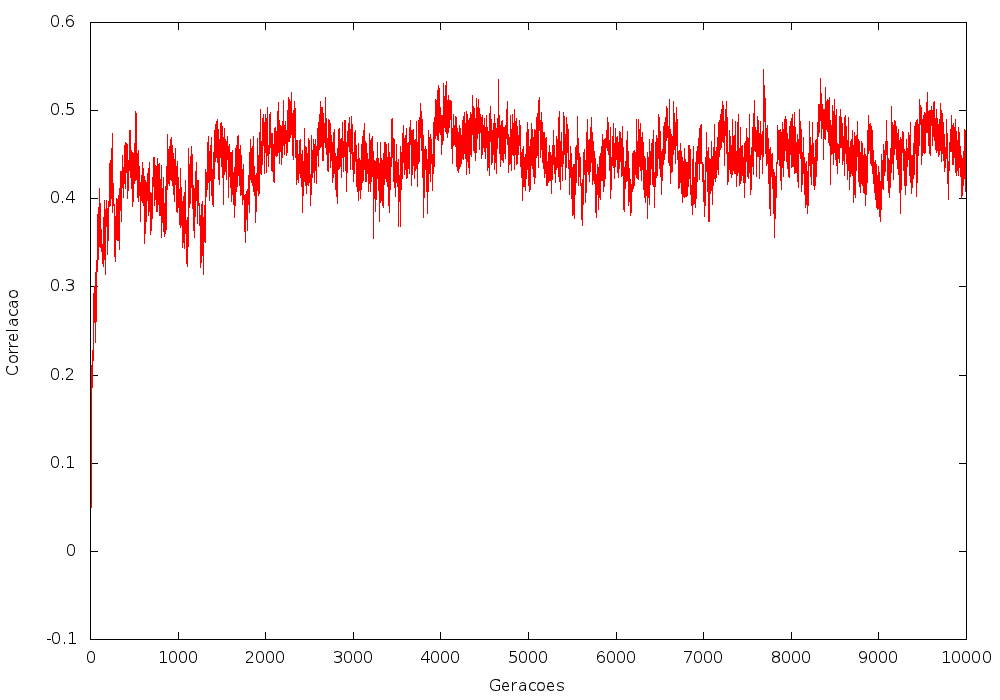
\includegraphics[width=150mm, height=80mm]{figuras/jones2tracos.png}
    \caption{Evolução da correlação entre dois caracteres ligados por efeitos
    mutacionais pleiotrópicos sobre seleção estabilizadora correlacionada.
    Nesta simulação $r_\omega=0.8$, $Ne=5.000$, $p=2$, $m=50$}
    \label{jones2tracos}
\end{figure}

Como nosso objetivo é expandir a modelagem para mais caracteres, em seguida
adicionamos um caráter ao sistema.
Nesse caso, as considerações sobre a dificuldade de manter a matriz
$\mathbf{M}$
positiva definida já se aplicam, sendo necessário fazer uso da correção
de autovalores.
Mesmo assim, o resultado é bastante semelhante, ainda com a correlação
entre os 3 caracteres se alinhando com a matriz $\pmb{\omega}$ (figuras
\ref{jones3tracos} e \ref{MatJones3tracos}).

\begin{figure}[htbp]
    \centering
    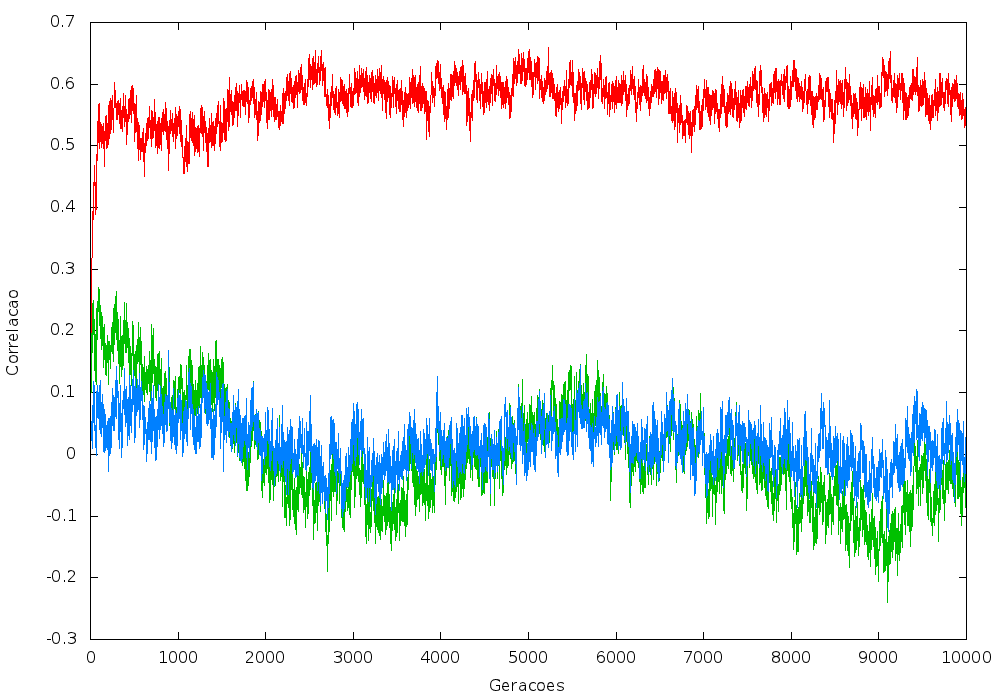
\includegraphics[width=150mm, height=80mm]{figuras/jones3tracos.png}
    \caption{Evolução da correlação entre três caracteres ligados por efeitos
        mutacionais pleiotrópicos sobre seleção estabilizadora correlacionada.
        A seleção propicia a integração entre dois caracteres (linha vermelha) e a desintegração
        desses dois com o terceiro (linhas azul e verde).
        Nesta simulação $r_\omega$ como na equação \ref{romega},
        $Ne=5.000$, $p=3$, $m=50$.}
    \label{jones3tracos}
\end{figure}

Na figura \ref{MatJones3tracos} vemos representações gráficas da matriz
de correlação fenotípica ao final da simulação e da matriz $\pmb{\omega}$ de
seleção estabilizadora correlacionada.
Caselas mais claras indicam correlação maior.
Nesse caso, a matriz de correlação da superfície de seleção foi:

\begin{equation}
    Corr(\pmb{\omega}) = \left( \begin{smallmatrix} 1 & 0.9 & 0.1\\  0.9 & 1 & 0.1 \\ 0.1 & 0.1 & 1 \end{smallmatrix}  \right)
    \label{romega}
\end{equation}

E a matriz de covariância da superfície de seleção: 

\begin{equation}
    \pmb{\omega} = \left( \begin{smallmatrix} 9 & 8.1 & 0.9\\  8.1 & 9 & 0.9 \\ 0.9 & 0.9 & 9 \end{smallmatrix}  \right)
\end{equation}

\begin{figure}[htbp]
    \centering
    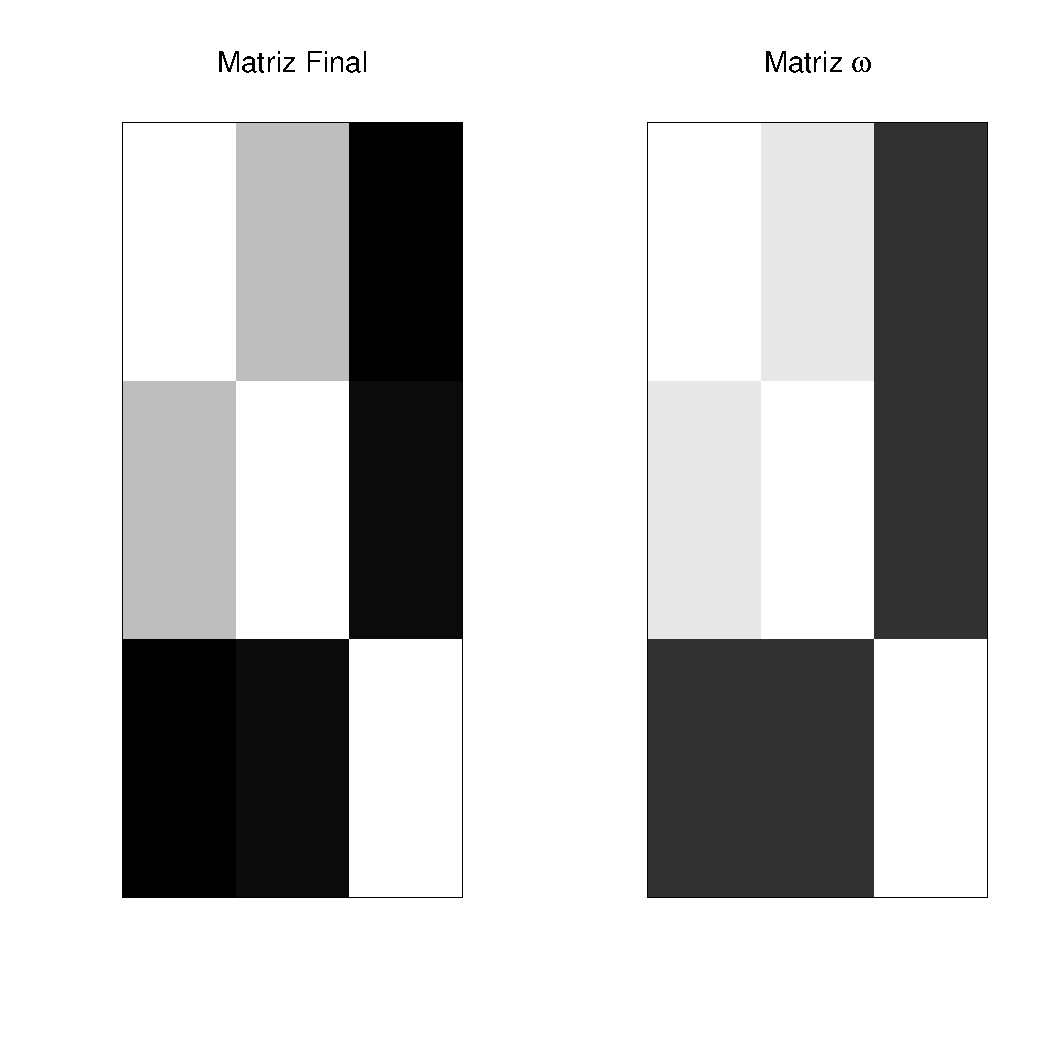
\includegraphics[width=150mm, height=80mm]{figuras/Mat3tracos}
    \caption{Comparação entre a matriz de correlação final para 3
        caracteres após 10.000 gerações de seleção e a matriz
        $\pmb{\omega}$ da superfície de seleção.}
    \label{MatJones3tracos}
\end{figure}

Quando procuramos ampliar o número de caracteres, porém, o alinhamento da
matriz $\mathbf{G}$ com a matriz $\pmb{\omega}$ se mostrou problemático.
Nesse caso a matriz de correlação da superfície de seleção continha dois
módulos, e era dada por:

\begin{equation}
    Corr(\pmb{\omega}) = \left( 
    \begin{smallmatrix} 
        1 & 0.8 & 0.8 & 0.8 & 0.8 & 0 & 0 & 0 & 0 & 0\\  
      0.8 & 1 & 0.8 & 0.8 & 0.8 & 0 & 0 & 0 & 0 & 0\\  
      0.8 & 0.8 & 1 & 0.8 & 0.8 & 0 & 0 & 0 & 0 & 0\\  
      0.8 & 0.8 & 0.8 & 1 & 0.8 & 0 & 0 & 0 & 0 & 0\\  
      0.8 & 0.8 & 0.8 & 0.8 & 1 & 0 & 0 & 0 & 0 & 0\\  
        0 & 0 & 0 & 0 & 0 & 1 & 0.8 & 0.8 & 0.8 & 0.8\\ 
        0 & 0 & 0 & 0 & 0 & 0.8 & 1 & 0.8 & 0.8 & 0.8\\
        0 & 0 & 0 & 0 & 0 & 0.8 & 0.8 & 1 & 0.8 & 0.8\\
        0 & 0 & 0 & 0 & 0 & 0.8 & 0.8 & 0.8 & 1 & 0.8\\
        0 & 0 & 0 & 0 & 0 & 0.8 & 0.8 & 0.8 & 0.8 & 1
    \end{smallmatrix}  \right)
    \label{matw}
\end{equation}

Na figura \ref{jones10tracos} vemos a trajetória típica das correlações
fenotípicas com uma matriz $\pmb{\omega}$ com dois módulos (ver figura
\ref{MatJones10tracos}).  
Aqui não existe mais a distinção entre
correlações dentro de módulos (altas) e entre módulos (baixas).
Os resultados da evolução da modularidade $L$ e do AVG-Ratio confirmam a
ausência de modularidade no sistema.
A modularidade $L$ apresenta uma leve subida ao longo da simulação, mas
o AVG-Ratio permanece estável (Figura \ref{jones10tracosStats}).
Isso se deve à modularidade $L$ capturar qualquer tipo de modularidade
na matriz, não só aquela associada a superfície de seleção.
Na figura \ref{MatJones10tracos} fica claro que não existe semelhança
entre as matrizes $\mathbf{G}$ e $\pmb{\omega}$.
Realizamos essas simulações com uma gama grande de intensidades de
seleção e chegando até 100.000 gerações de seleção, sem nenhum indício de
alinhamento estável entre as matrizes $\mathbf{G}$ e $\pmb{\omega}$.  

\begin{figure}[htbp]
    \centering
    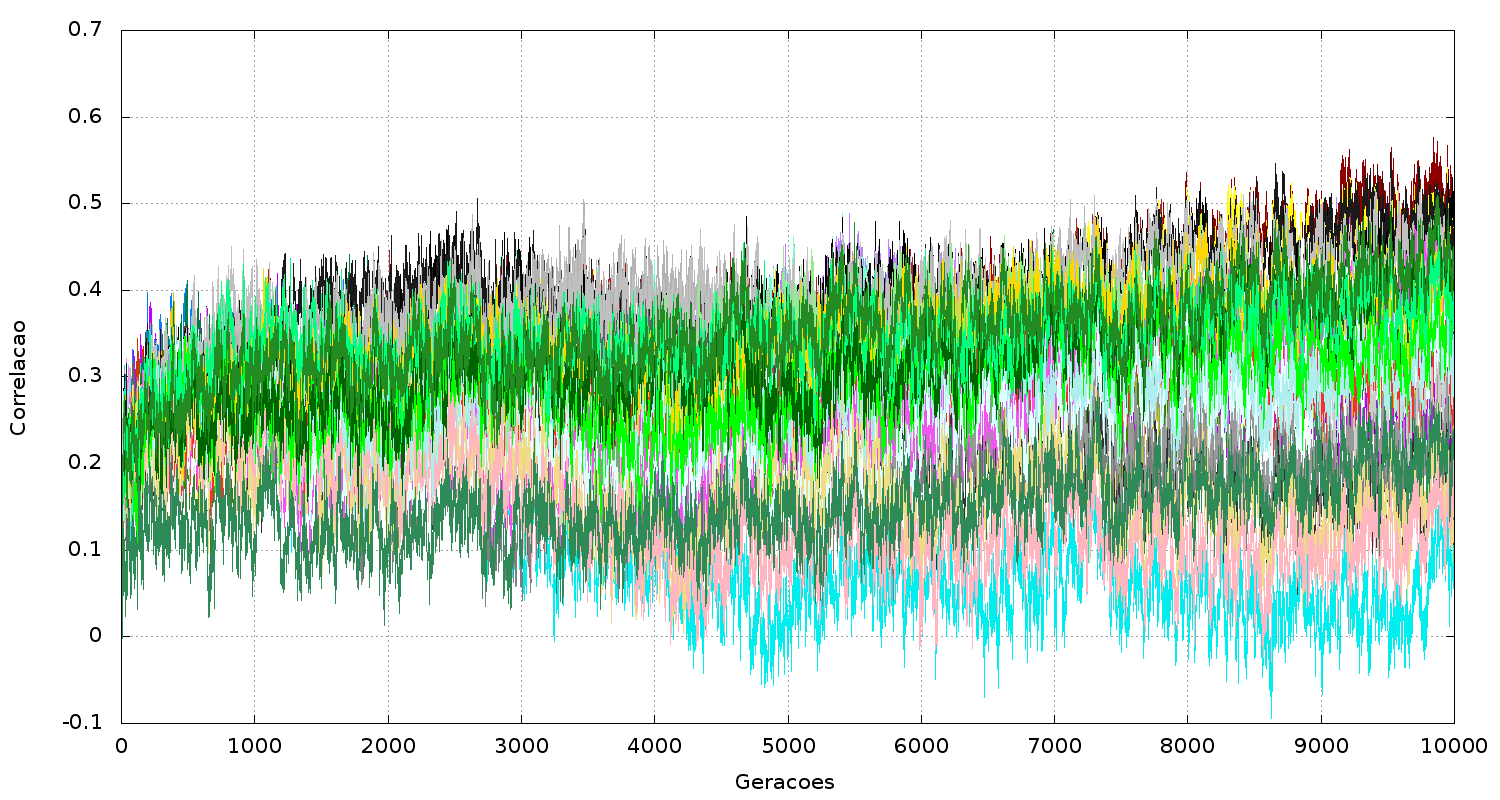
\includegraphics[width=150mm, height=80mm]{figuras/jones10tracos.png}
    \caption{Evolução da correlação entre dez caracteres ligados por efeitos
        mutacionais pleiotrópicos sobre seleção estabilizadora
        correlacionada. Apesar da seleção promover a integração entre os
        5 primeiros e os 5 últimos caracteres e a desintegração entre esse
        módulos, isso não se transmite à matriz de correlação. Nesta simulação
        $r_\omega$ como na equação \ref{matw}, $Ne=5.000$, $p=10$, $m=50$.}
    \label{jones10tracos}
\end{figure}

\begin{figure}[htbp]
    \centering
    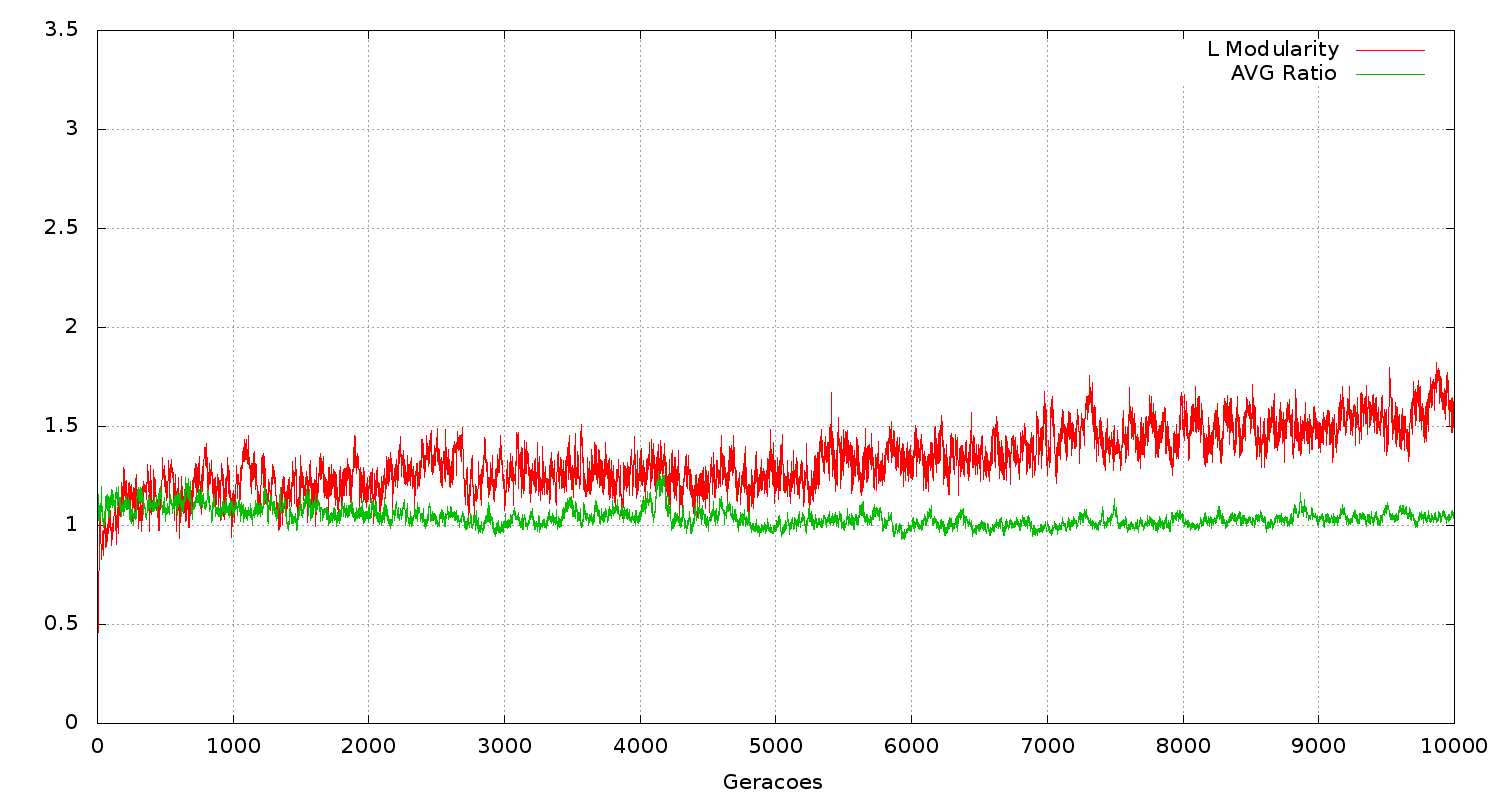
\includegraphics[width=150mm, height=80mm]{figuras/jones10tracosStats.png}
    \caption{Evolução da modularidade $L$ e AVG-Ratio para as matrizes de
    correlação representadas na figura \ref{jones10tracos}}
    \label{jones10tracosStats}
\end{figure}

\begin{figure}[htbp]
    \centering
    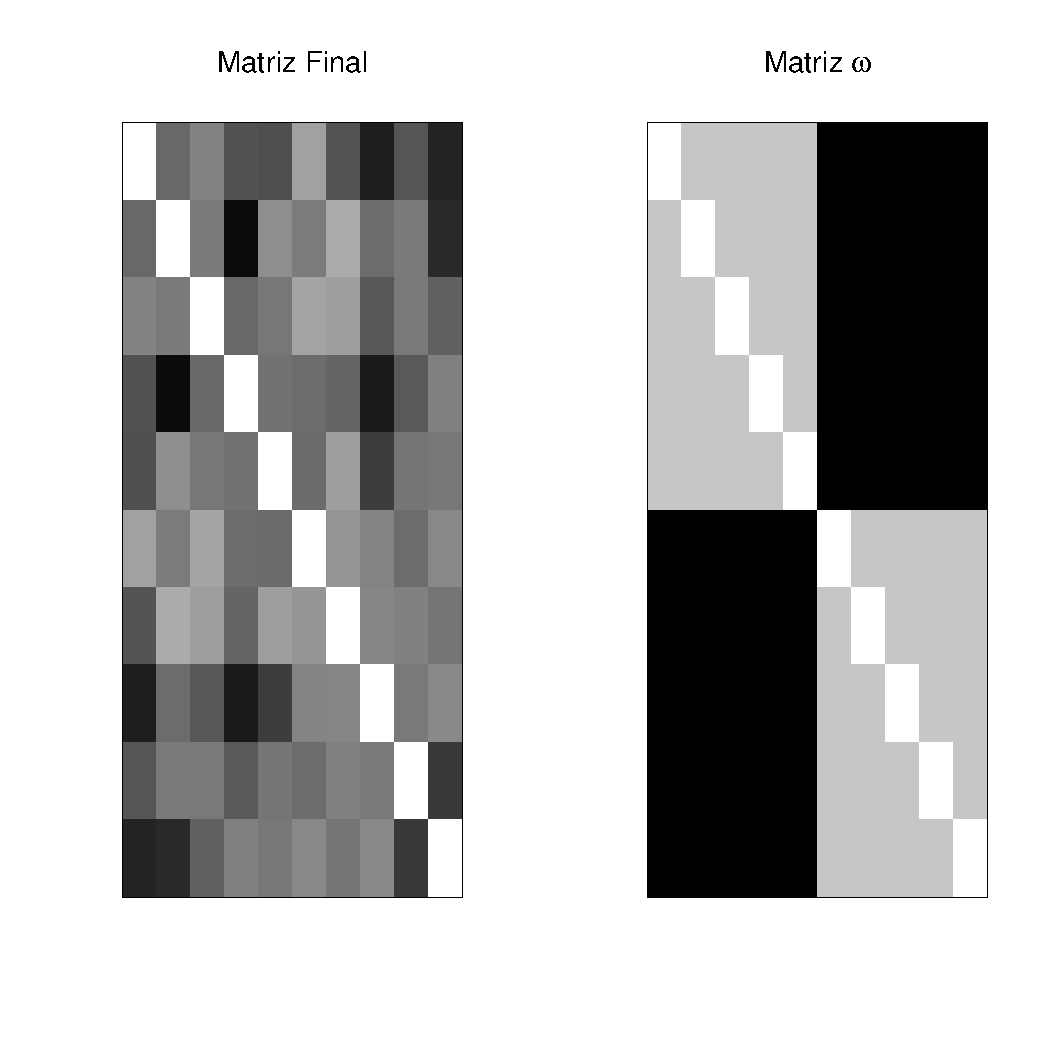
\includegraphics[width=150mm, height=80mm]{figuras/Mat10tracos}
    \caption{Comparação entre a matriz de correlação final para 10
        caracteres após 10.000 gerações de seleção representadas na figura
    \ref{jones10tracos} e a matriz $\pmb{\omega}$ da superfície de seleção.}
    \label{MatJones10tracos}
\end{figure}

\subsection{Seleção Direcional}

Em seguida, procuramos explorar como a inclusão de seleção direcional afetaria o
alinhamento das matrizes $\mathbf{G}$ e $\pmb{\omega}$.
Utilizamos novamente uma matriz $\pmb{\omega}$ modular e acrescentamos seleção
direcional correlacionada, de mudança conjunta na média dos caracteres
dentro de cada um dos módulos, e mudanças antagônicas entre módulos.
Ou seja, os 5 primeiros caracteres tiveram seu ótimo fenotípico aumentado a
uma taxa constante e os 5 últimos caracteres tiveram seu ótimo reduzido de
forma simétrica ($\Delta_S=0.2$).
As populações respondem a essa seleção de forma eficiente, alterando
suas médias de acordo com a posição do ótimo.
Após 10.000 gerações de seleção direcional, observamos a matriz final
e a evolução de todas as correlações genéticas nesse período.
Os resultados podem ser vistos nas figuras \ref{jones10tracosDirecional}
, \ref{jones10tracosDirecionalStats} e \ref{MatJones10tracosDirecional}.
Mesmo nessas condições, não observamos a emergência de módulos
variacionais na matriz $\mathbf{G}$, que indicaria semelhança com a matriz $\pmb{\omega}$
e o padrão de seleção direcional correlacionada.

\begin{figure}[htbp]
    \centering
    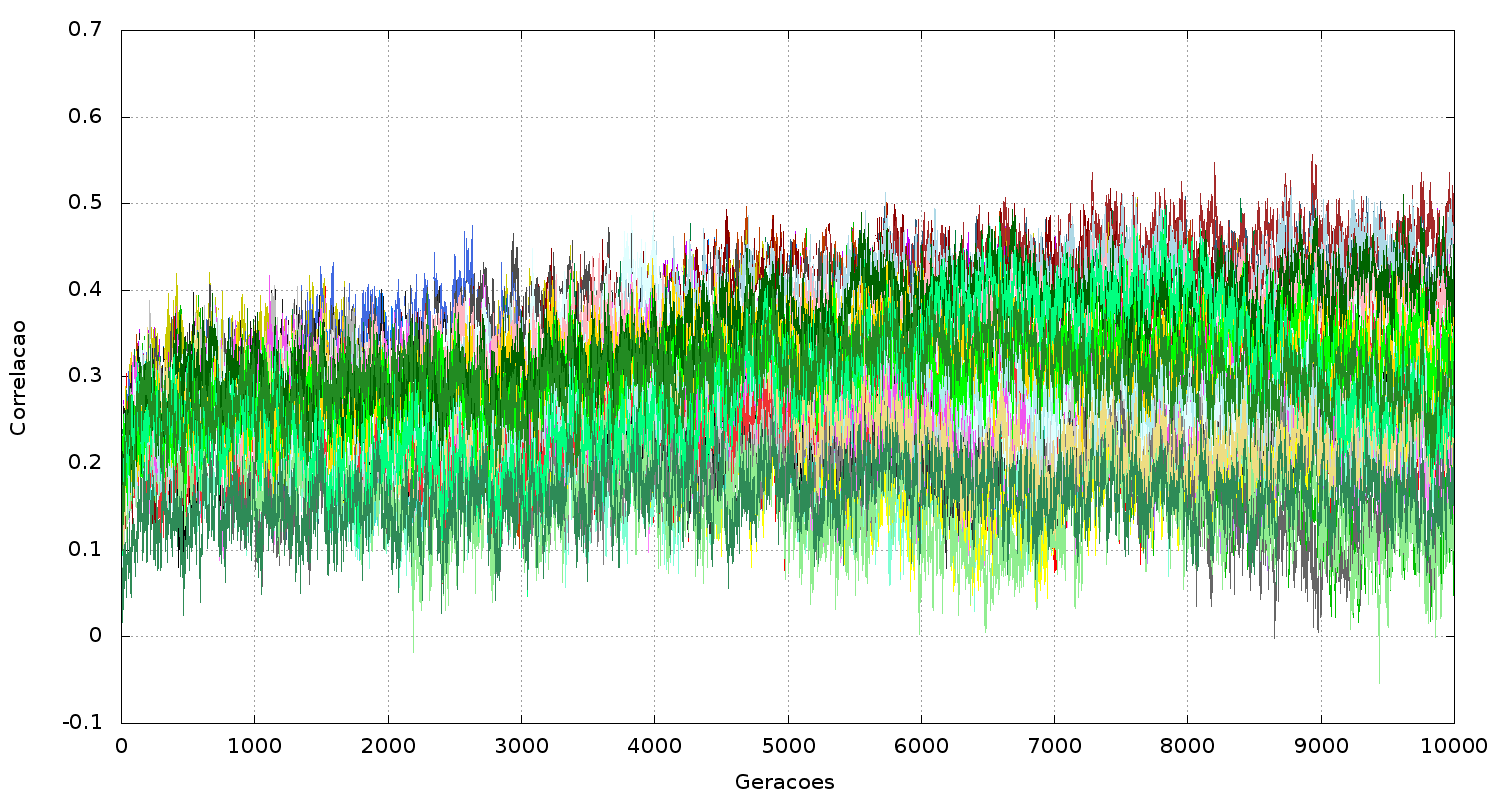
\includegraphics[width=150mm, height=80mm]{figuras/jones10tracosDirecional.png}
    \caption{Evolução da correlação entre dez caracteres ligados por efeitos
        mutacionais pleiotrópicos sobre seleção estabilizadora correlacionada
        e seleção direcional intensa para mudança correlacionada dentro dos
    módulos. Novamente, isso não se traduz na matriz de correlação genética.}
    \label{jones10tracosDirecional}
\end{figure}

\begin{figure}[htbp]
    \centering
    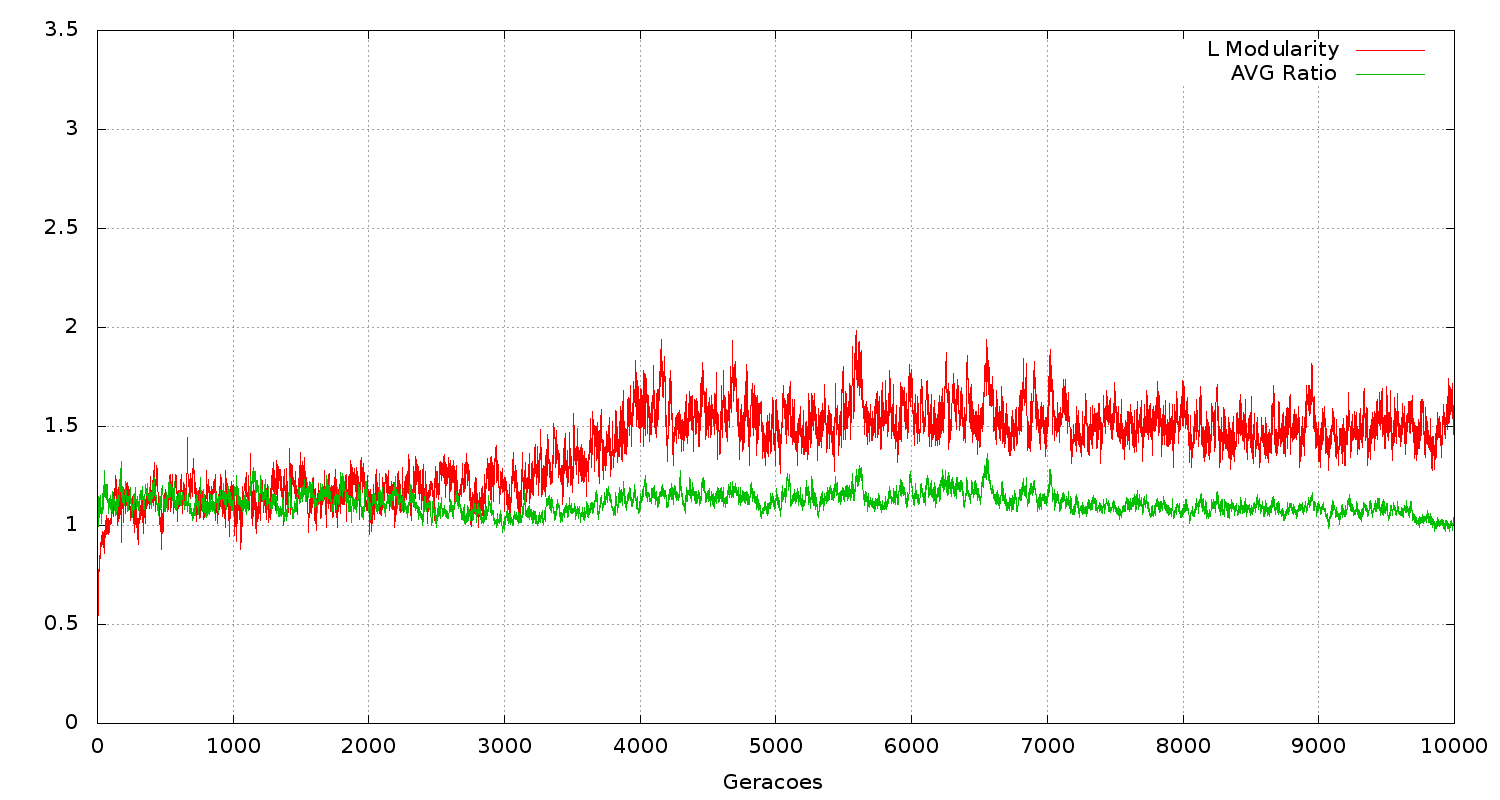
\includegraphics[width=150mm, height=80mm]{figuras/jones10tracosDirecionalStats.png}
    \caption{Evolução da modularidade $L$ e AVG-Ratio para as matrizes de
    correlação representadas na figura \ref{jones10tracosDirecional}}
    \label{jones10tracosDirecionalStats}
\end{figure}

\begin{figure}[htbp]
    \centering
    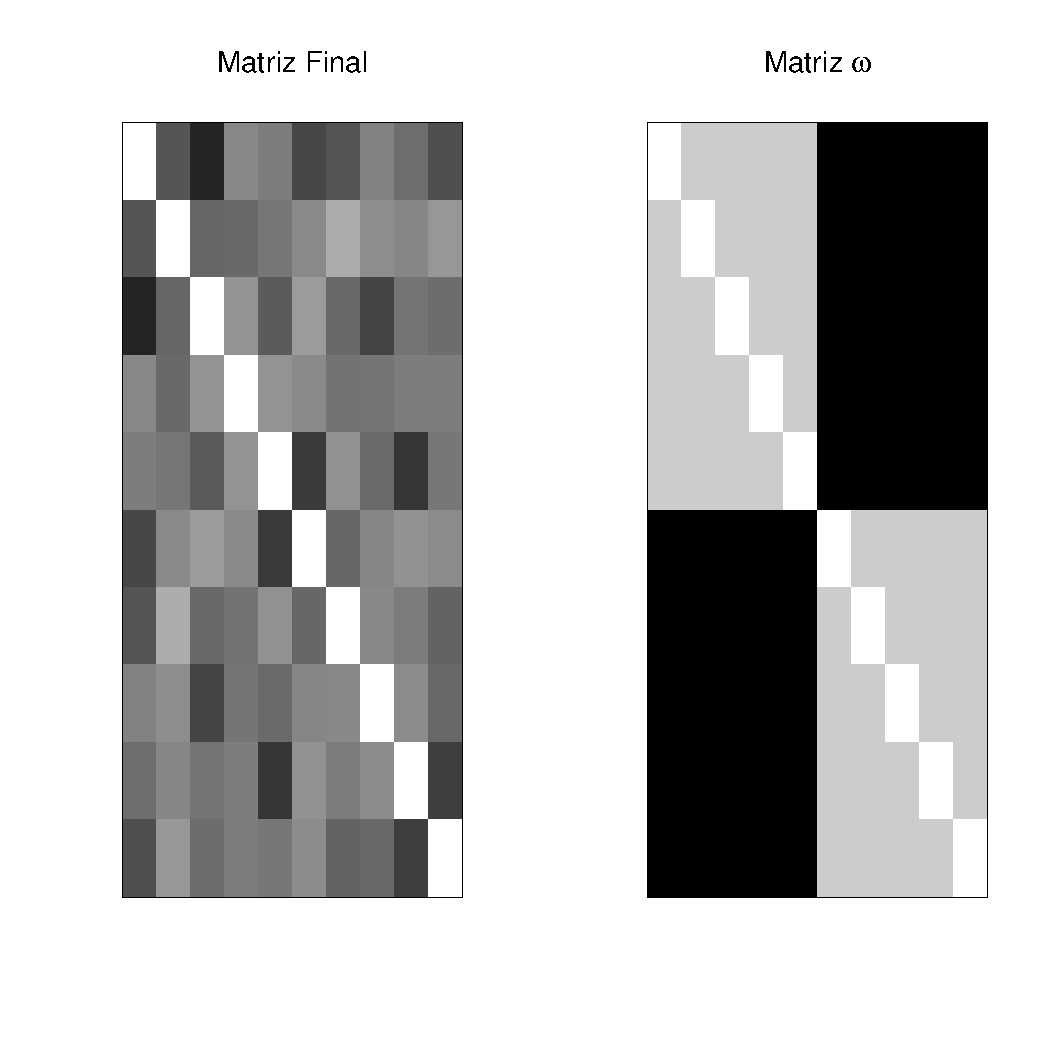
\includegraphics[width=150mm, height=80mm]{figuras/Mat10tracosDirecional}
    \caption{Comparação entre a matriz de correlação final para 10 caracteres
        após 10.000 gerações de seleção direcional e estabilizadora
        representadas na figura \ref{jones10tracosDirecional} com a matriz
    $\pmb{\omega}$ da superfície de seleção.}
    \label{MatJones10tracosDirecional}
\end{figure}

Acreditamos que essa dificuldade em reproduzir os resultados encontrados
em sistemas com 2 e 3 caracteres no sistema com 10 caracteres se deve ao aumento
considerável do espaço possível de variação que a inclusão de cada novo
caráter representa.
O morfoespaço cresce rapidamente com a inclusão de cada novo caráter, e
o espaço permitido para a matriz $\mathbf{M}$ também.
A seleção indireta, então, se torna muito fraca para promover o
alinhamento entre as matrizes, provavelmente porque as mutações nos
alelos mutacionais não exploram de forma adequada (ergódica) o espaço da
matriz mutacional, levando a uma situação de não alinhamento mesmo com
uma pressão seletiva considerável.
Outro problema é a técnica de extensão utilizada para gerar matrizes
positivas definidas.
Apesar de gerar matrizes similares às criadas diretamente dos alelos
mutacionais, qualquer modificação na matriz diminui a semelhança entre
matrizes de uma geração para outra, e introduz ruido na herança.
Em outras palavras, a semelhança da própria matriz $\mathbf{M}$ de um
geração para a outra, definida através de alelos mutacionais aditivos,
diminui com o aumento da dimensionalidade do sistema e impossibilita que
seleção atue de forma eficiente na sua estrutura, tanto pelo aumento da
dimensionalidade quanto pelas correções necessárias para tornar a matriz
bem definida.
Talvez outros esquemas de simulação para matrizes de mutação herdáveis,
definidas para cada indivíduo separadamente, variáveis e sujeitas à
seleção natural, venham a sanar essa limitação.
O uso de correlações parciais para gerar as matrizes mutacionais, por
exemplo, evita o problema da geração de matrizes não positivas
definidas \citep{Joe2006, Lewandowski2009}, e pode ser uma saída
interessante para o modelo com matriz $\mathbf{M}$ em muitas dimensões.
Pretendemos explorar essa solução no futuro.

\section{Resultados e Discussão $\cdot$ Matriz $\mathbf{B}$}

Todas as simulações dessa seção começam com o mesmo estado inicial, com
a matriz $\mathbf{B}$ totalmente formada por $1$, ou seja, integração total, e
todos os valores aditivos $0$, ou seja, todos os caracteres determinados
apenas por efeitos ambientais e com sua porção aditiva igual a zero.
As primeiras gerações são dependentes desses estado inicial e não trazem
informação.
Após cerca de $2.000$ gerações o sistema se encontra em equilíbrio
seleção-mutação-deriva e pode ser analisado independentemente do estado
inicial.
Isso se reflete em todos os gráficos como um transiente instável, seguido
de estabilidade dependente principalmente do tamanho populacional.
Discutimos esses efeitos e outros na próxima seção.

\subsection{Seleção Estabilizadora}

No segundo tipo de modelagem, começamos já com 10 caracteres sofrendo
seleção estabilizadora correlacionada dada pela matriz apresentada na
equação \ref{matw}.
Exploramos então a influência de várias razões entre a taxa de mutação
nos efeitos genéticos ($\mu$) e a taxa de mutação nas caselas da matriz
$\mathbf{B}$ ($\mu_B$).
Essa razão $\mu/\mu_B$ define como será a dinâmica temporal de mudança
entre dois níveis: o dos efeitos genéticos e o da atribuição desses
efeitos à porção aditiva dos caracteres quantitativos, que chamamos aqui de efeito {\it
ontogenético}, incluindo também todos os efeitos pleiotrópicos e
epistáticos dos loci sobre o fenótipo.
Conforme vemos nas figuras \ref{MatBEstab} e \ref{EstabRMuStats}, apesar de mudanças na
magnitude das correlações com o aumento da razão $\mu/\mu_B$, não
observamos o surgimento de módulos variacionais apenas com seleção
estabilizadora correlacionada.

\begin{figure}[htbp]
    \centering
    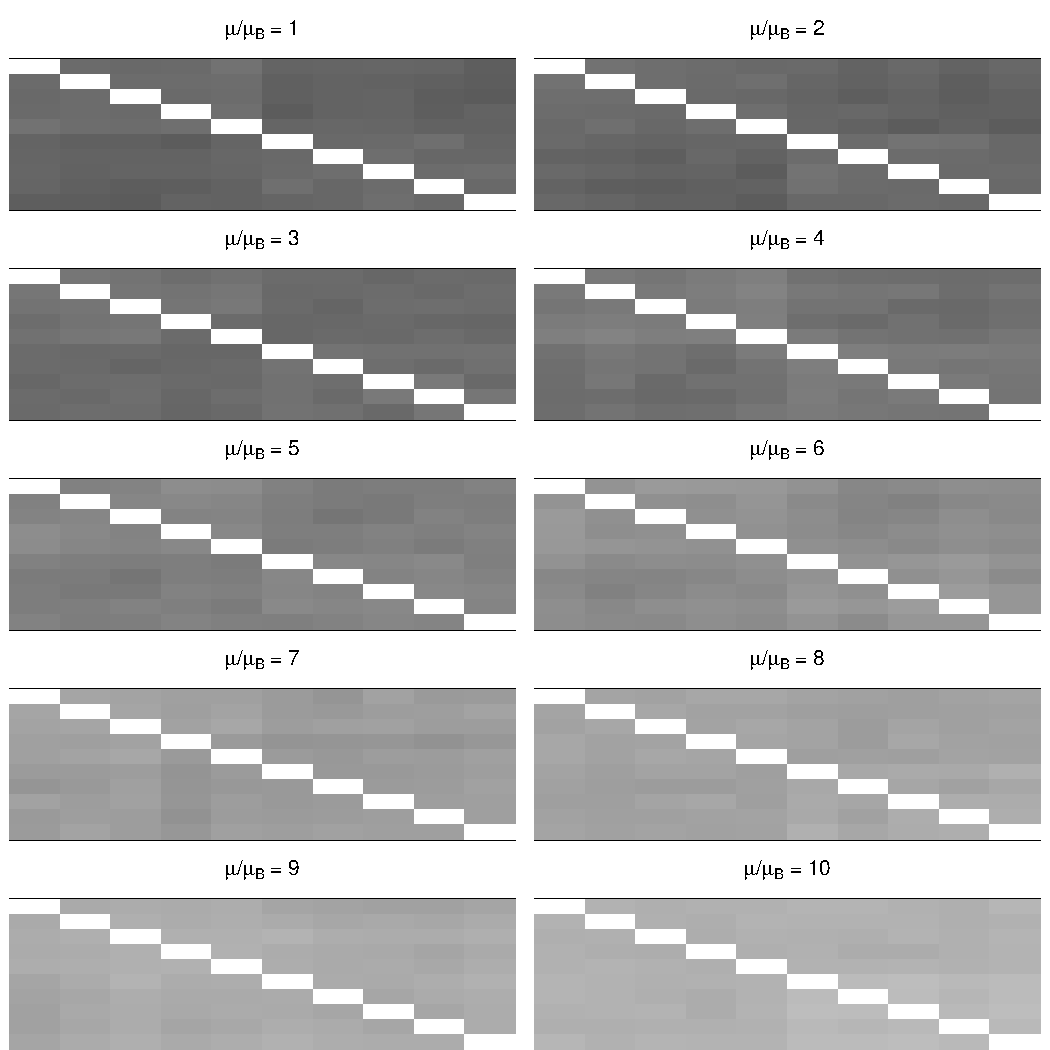
\includegraphics[width=150mm, height=180mm]{figuras/MatBEstabRMu}
    \caption{Matriz final média de 10 corridas para diferentes razões de
        $\mu$ e $\mu_B$, com seleção estabilizadora correlacionada com 2
    módulos.}
    \label{MatBEstab}
\end{figure}

\begin{figure}[htbp]
    \centering
    \subfloat [$\mu/\mu_B = 1$]{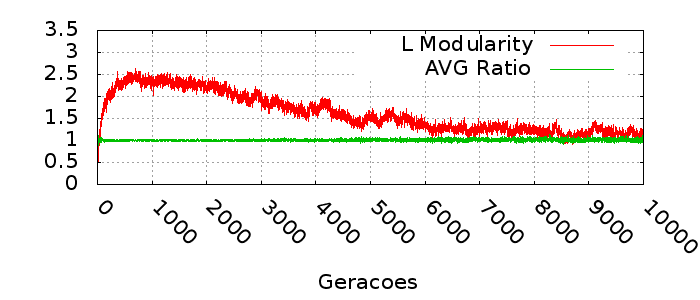
\includegraphics[width=70mm, height=30mm]{figuras/EstabRMuStats1.png}}\vspace{11pt}
    \subfloat [$\mu/\mu_B = 2$]{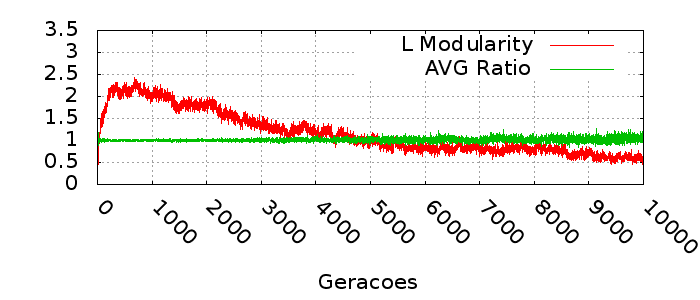
\includegraphics[width=70mm, height=30mm]{figuras/EstabRMuStats2.png}}\\ 
    \vspace{-18pt}
    \subfloat [$\mu/\mu_B = 3$]{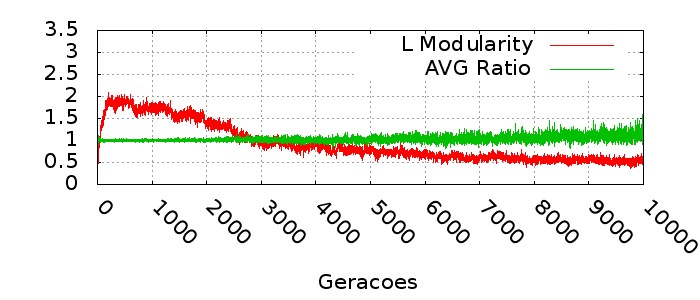
\includegraphics[width=70mm, height=30mm]{figuras/EstabRMuStats3.png}}\vspace{11pt} 
    \subfloat [$\mu/\mu_B = 4$]{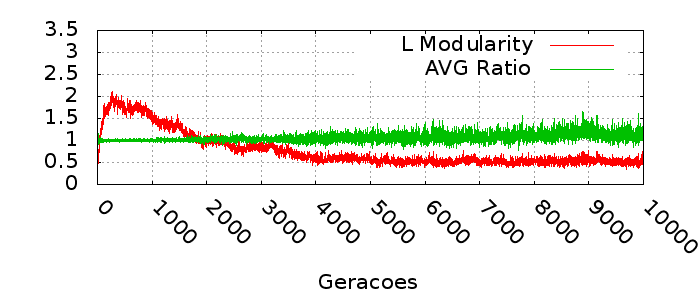
\includegraphics[width=70mm, height=30mm]{figuras/EstabRMuStats4.png}}\\
    \vspace{-18pt}
    \subfloat [$\mu/\mu_B = 5$]{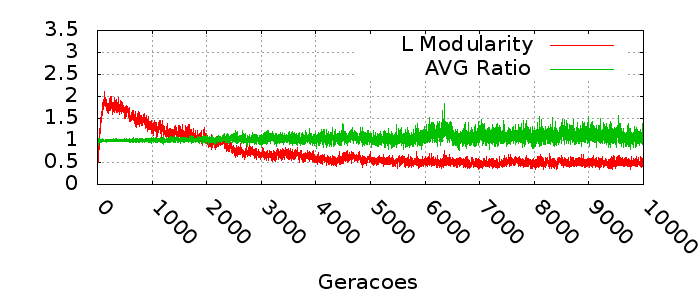
\includegraphics[width=70mm, height=30mm]{figuras/EstabRMuStats5.png}}\vspace{11pt}
    \subfloat [$\mu/\mu_B = 6$]{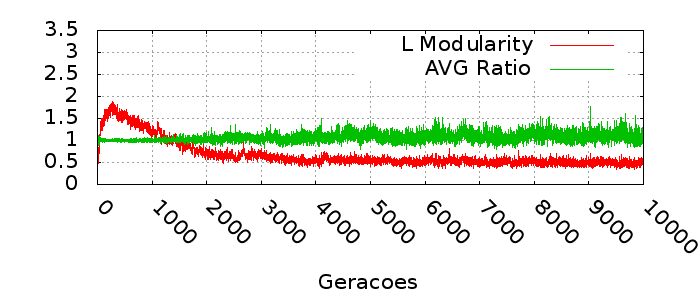
\includegraphics[width=70mm, height=30mm]{figuras/EstabRMuStats6.png}}\\
    \vspace{-18pt}
    \subfloat [$\mu/\mu_B = 7$]{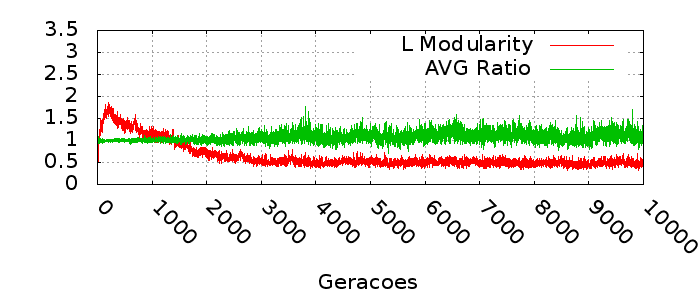
\includegraphics[width=70mm, height=30mm]{figuras/EstabRMuStats7.png}}\vspace{11pt}
    \subfloat [$\mu/\mu_B = 8$]{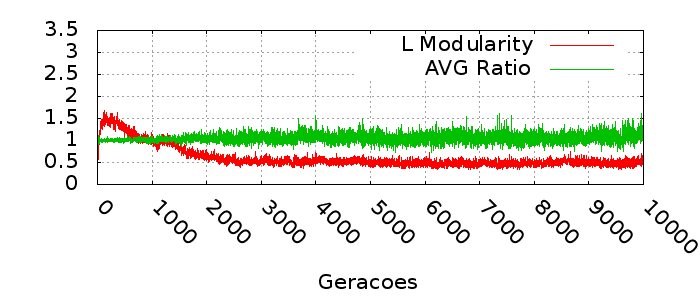
\includegraphics[width=70mm, height=30mm]{figuras/EstabRMuStats8.png}}\\
    \vspace{-18pt}
    \subfloat [$\mu/\mu_B = 9$]{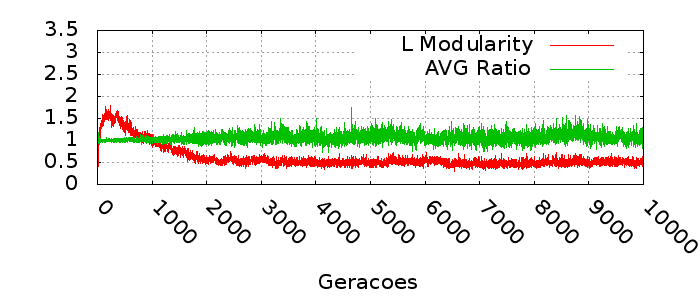
\includegraphics[width=70mm, height=30mm]{figuras/EstabRMuStats9.png}}\vspace{11pt}
    \subfloat [$\mu/\mu_B = 10$]{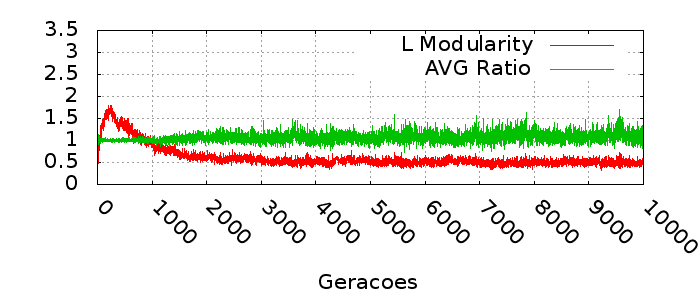
\includegraphics[width=70mm, height=30mm]{figuras/EstabRMuStats10.png}}\\
    \caption{Evolução típica de AVG-Ratio e modularidade $L$ para diferentes razões de
    $\mu$ e $\mu_B$, com seleção estabilizadora correlacionada com 2 módulos.}
    \label{EstabRMuStats}
\end{figure}

\subsection{Seleção Direcional}
\label{cap3:DirecB}

Com a inclusão de seleção direcional divergente, ou seja, para aumento
dos $5$ primeiros caracteres e diminuição dos $5$ últimos, como na
figura \ref{MatJones10tracosDirecional}, e $\mu/\mu_B = 0.1$, ainda não
observamos a formação de módulos na matriz $\mathbf{G}$ (figura
\ref{RMu01}).
Porém, como vemos na figura \ref{MatBDirecional-RMu}, o aumento  da
razão $\mu/\mu_B$ aliada à seleção direcional é capaz de alterar esse
comportamento.
Esse aumento parece promover um sistema capaz de responder de forma
eficiente às pressões seletivas impostas e gerar uma matriz $\mathbf{G}$ com a
estrutura modular privilegiada pela seleção estabilizadora e direcional.
Lembramos que na ausência de seleção direcional esse efeito não é
observado, mesmo com as mesmas razões $\mu/\mu_B$.
Na figura \ref{DirecionalRMuStats} vemos que razões baixas de $\mu/\mu_B$ levam
a sistemas bastante instáveis, apesar de modulares.
Isso pode ser interpretado como uma consequência de taxas de mudança em
cada nível da simulação incompatíveis com populações estáveis, pois as
mudanças {\it ontogenéticas} da matriz $\mathbf{B}$ não podem se dar na
mesma escala temporal das mudanças nos efeitos genéticos, ou o sistema
não tem tempo de responder à seleção de forma estável.

Para $\mu/\mu_B=1$, ou seja, com a taxa de mutação igual nos níveis
genético e ontogenético, o valor de modularidade $L$ flutua violentamente entre
as gerações, sugerindo uma modularidade muito instável.
Além disso, para valores de baixos de $\mu/\mu_B$ as correlações entre
os caracteres são extremamente baixas, em torno de $0$ entre módulos e
por volta de $0.2$ dentro de módulos.
A partir de $\mu/\mu_B=4$ o sistema se torna muito mais estável e
progressivamente menos modular.
Nós optamos por utilizar o valor $\mu/\mu_B=5$ nas simulações
subsequentes.
Essa opção se deu por uma série de fatores: nesse valor o sistema ainda
apresenta um aumento de modularidade ao longo das gerações; as
correlações aumentam para cerca de $0.2$ entre módulos e $0.4$ dentro de
módulos ao final da simulação; os valores de modularidade $L$ e
AVG-Ratio são bastante concordantes, sugerindo que os módulos
favorecidos pela seleção estão efetivamente sendo expressos na
população; e, por último, o sistema possui uma estabilidade razoável sem
se tornar incapaz de responder à seleção direcional.

\begin{figure}[htbp]
    \centering
    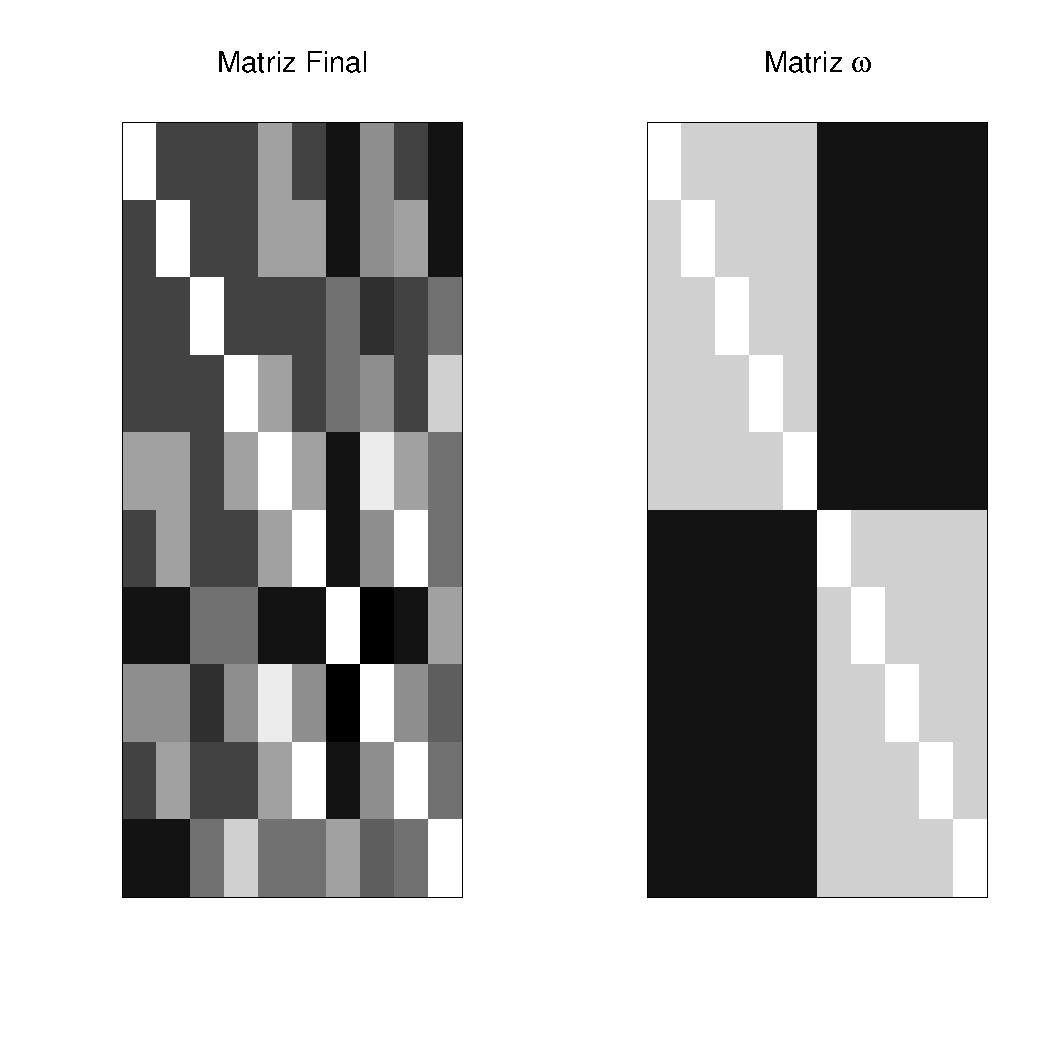
\includegraphics[width=150mm, height=80mm]{figuras/RMu01Omega}
    \caption{Comparação entre a matriz de correlação final média de 10
        corridas para o 10 caracteres após 10.000 gerações de seleção direcional e
        estabilizadora com a matriz $\pmb{\omega}$ da superfície de seleção e
    $\frac{\mu}{\mu_B}=0.1$, $Ne=2.500$, $\Delta_S=0.2$, $m/p=2$}
    \label{RMu01}
\end{figure}

Na figura \ref{MatBDirecionalNe2500RMu5} vemos um exemplo de corrida com
$N_e = 2.500$ e $\mu/\mu_B=5$, mostrando claramente a separação de grupos
de correlação dentro de e entre módulos.
Posteriormente vamos explorar a influência do tamanho populacional na
estabilidade das matrizes geradas pelas nossas simulações (figura
\ref{posselecao}).

\begin{figure}[htbp]
    \centering
    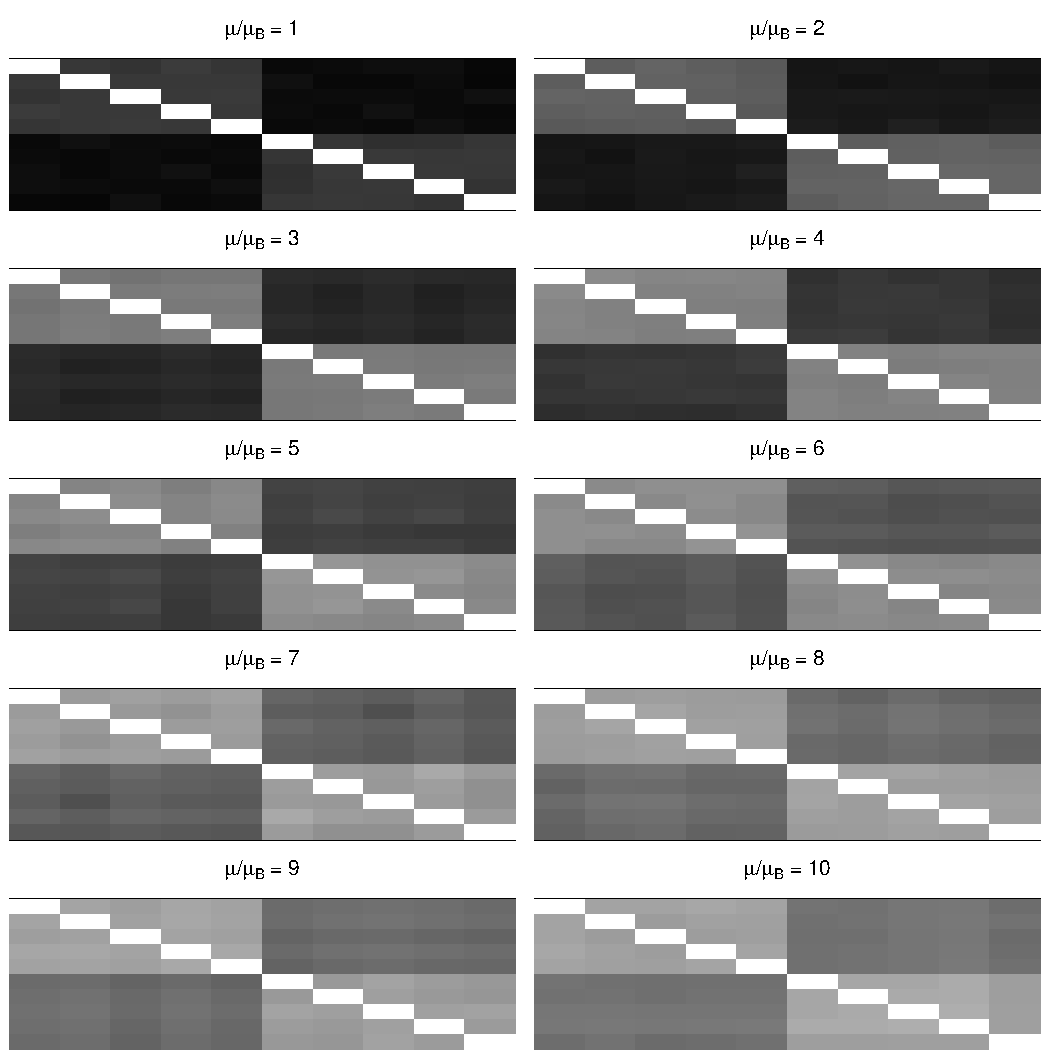
\includegraphics[width=150mm, height=180mm]{figuras/MatBDirecRMu}
    \caption{Matriz final média de 10 corridas para diferentes razões de
        $\frac{\mu}{\mu_B}$, com seleção estabilizadora correlacionada com 2
        módulos e seleção direcional correlacionada favorecendo os mesmos
    módulos. ($N_e=2.500$, $\Delta_S=0.2$, $m/p=2$)}
    \label{MatBDirecional-RMu}
\end{figure}

\begin{figure}[htbp]
    \centering
    \subfloat [$\mu/\mu_B = 1$]{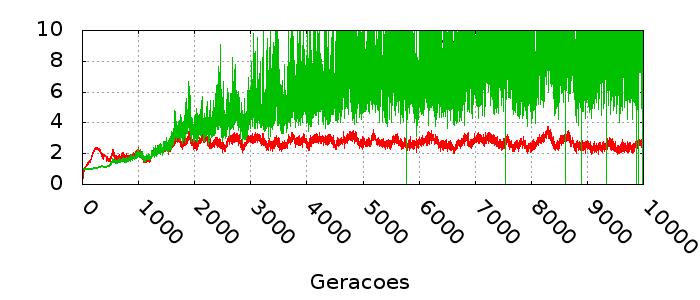
\includegraphics[width=70mm, height=30mm]{figuras/DirecionalRMuStats1.png}}\vspace{11pt}
    \subfloat [$\mu/\mu_B = 2$]{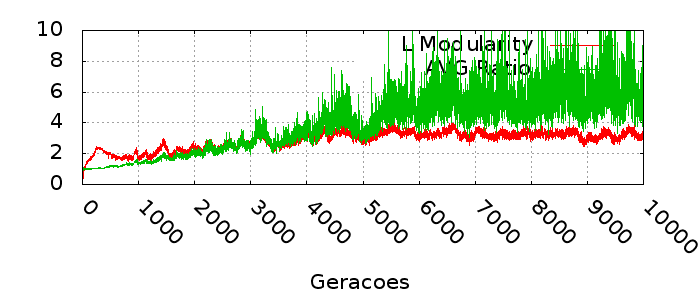
\includegraphics[width=70mm, height=30mm]{figuras/DirecionalRMuStats2.png}}\\ 
    \vspace{-18pt}
    \subfloat [$\mu/\mu_B = 3$]{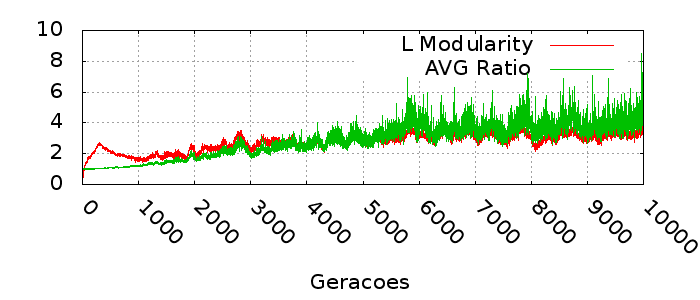
\includegraphics[width=70mm, height=30mm]{figuras/DirecionalRMuStats3.png}}\vspace{11pt} 
    \subfloat [$\mu/\mu_B = 4$]{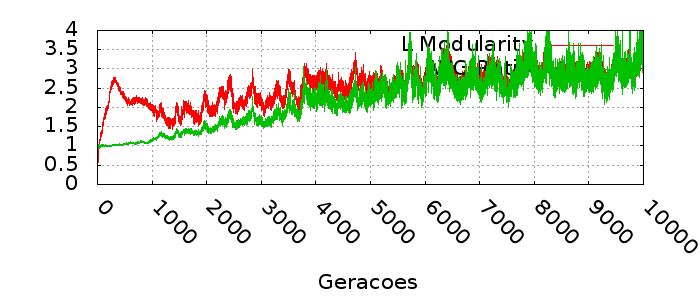
\includegraphics[width=70mm, height=30mm]{figuras/DirecionalRMuStats4.png}}\\
    \vspace{-18pt}
    \subfloat [$\mu/\mu_B = 5$]{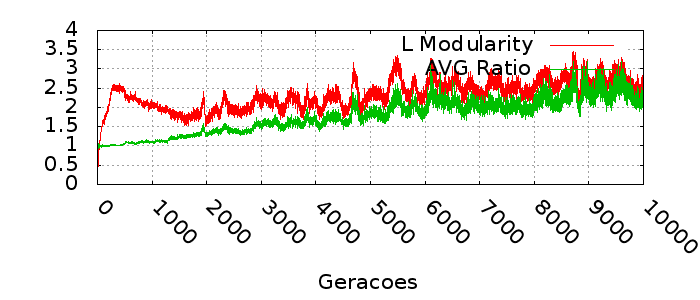
\includegraphics[width=70mm, height=30mm]{figuras/DirecionalRMuStats5.png}}\vspace{11pt}
    \subfloat [$\mu/\mu_B = 6$]{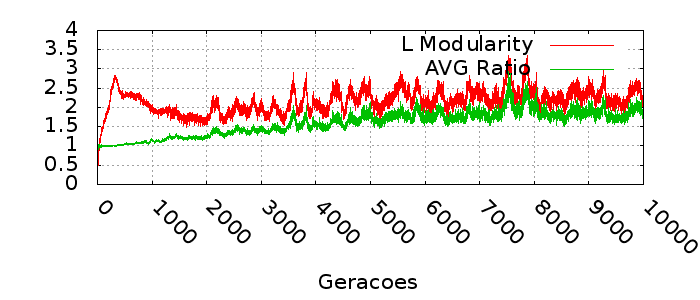
\includegraphics[width=70mm, height=30mm]{figuras/DirecionalRMuStats6.png}}\\
    \vspace{-18pt}
    \subfloat [$\mu/\mu_B = 7$]{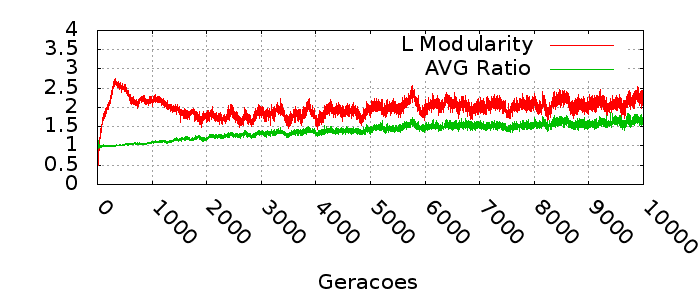
\includegraphics[width=70mm, height=30mm]{figuras/DirecionalRMuStats7.png}}\vspace{11pt}
    \subfloat [$\mu/\mu_B = 8$]{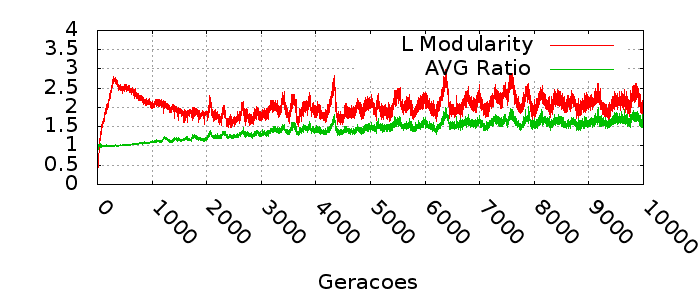
\includegraphics[width=70mm, height=30mm]{figuras/DirecionalRMuStats8.png}}\\
    \vspace{-18pt}
    \subfloat [$\mu/\mu_B = 9$]{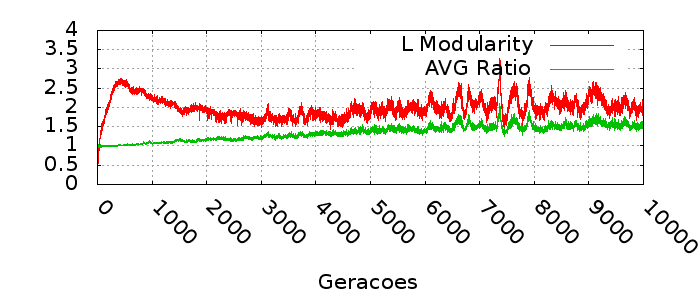
\includegraphics[width=70mm, height=30mm]{figuras/DirecionalRMuStats9.png}}\vspace{11pt}
    \subfloat [$\mu/\mu_B = 10$]{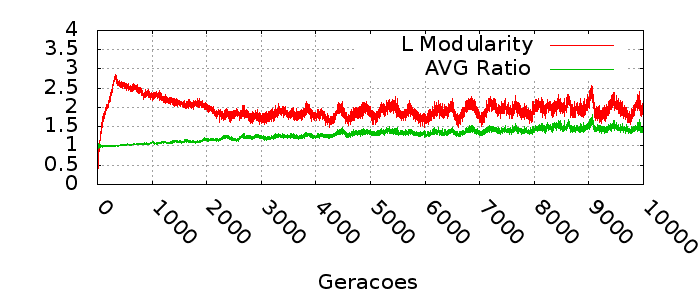
\includegraphics[width=70mm, height=30mm]{figuras/DirecionalRMuStats10.png}}\\
    \caption{Evolução típica de AVG-Ratio e modularidade $L$ para diferentes razões 
        $\mu/\mu_B$, com seleção estabilizadora correlacionada com 2
        módulos e seleção direcional correlacionada favorecendo os mesmos
    módulos. Atenção para a mudança de escala nos eixos verticais. ($N_e=2.500$, $\Delta_S=0.2$, $m/p=2$)}
    \label{DirecionalRMuStats}
\end{figure}

\begin{figure}[htbp]
    \centering
    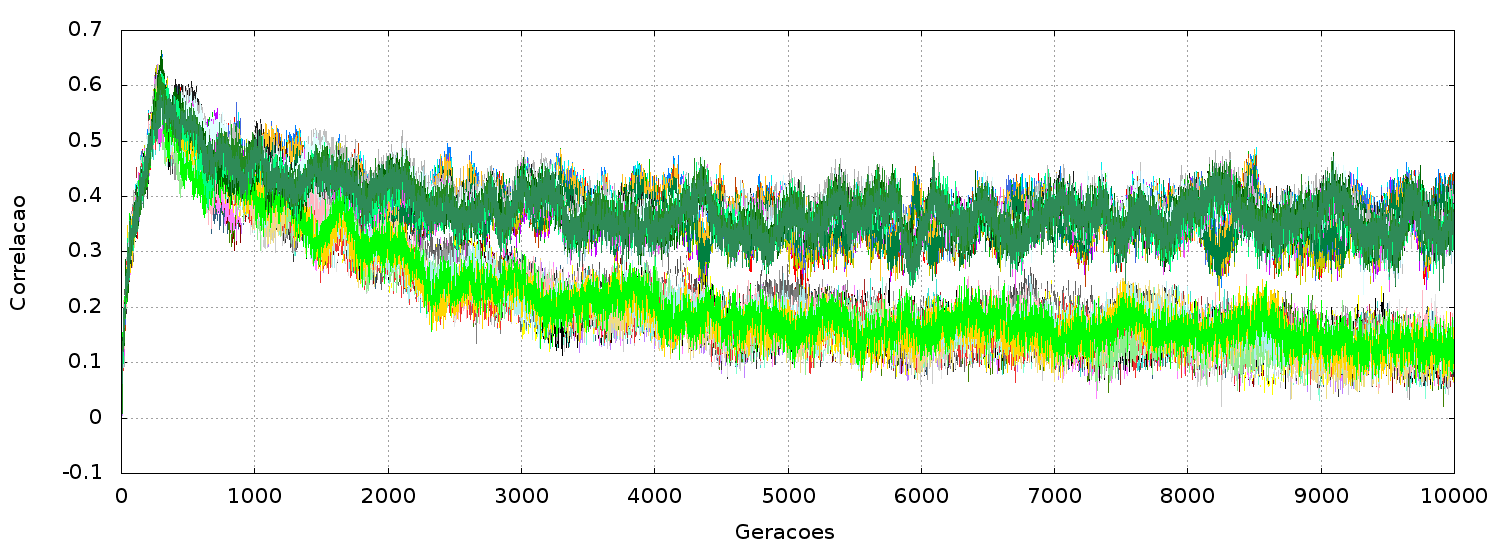
\includegraphics[width=150mm, height=55mm]{figuras/direcionalRMu5Ne2500IntSel200.png}
    \caption{Evolução da correlação entre dez caracteres ligados por efeitos
        pleiotrópicos controlados por uma função ontogenética linear binária
        variável, sofrendo seleção estabilizadora correlacionada
        e seleção direcional intensa para mudança correlacionada dentro dos
        módulos durante as 10.000 gerações.
    ($N_e = 2.500$, $\mu/\mu_B=5$, $\Delta_S=0.2$, $m/p=2$)}
    \label{MatBDirecionalNe2500RMu5}
\end{figure}

\subsection{Intensidade de Seleção Direcional}

Estamos interessados também na força de seleção direcional necessária
para gerar a estrutura modular nas matrizes de covariação.
Nas figuras \ref{MatBIntSel110} e \ref{MatBIntSel1120} vemos matrizes
médias finais para 10 corridas com $N_e = 1.000$, $\mu/\mu_B=5$ e
intensidade de seleção variável.
Para isso, modificamos o quanto o pico adaptativo era alterado para cada
caráter a cada geração, de $0.01$ até $0.2$ por geração durante 10.000
gerações.
Nas figuras \ref{IntSelStats10100} e \ref{IntSelStats110200} vemos
evoluções típicas de AVG-Ratio e modularidade $L$ para corridas com
várias intensidades de seleção, mostrando o quão estáveis e o quão
rápido os padrões modulares se estabelecem nessas condições.
Vemos que mesmo com um tamanho populacional considerável ($Ne = 2.500$)
ainda observamos flutuações grandes.

Quando aumentamos a intensidade de seleção, os módulos se tornam
mais evidentes, mas acima de uma certa intensidade ($\Delta_S \simeq 0.06$)
esse efeito se torna mais discreto.
Esse platô na resposta à seleção direcional pode ser explicado por como
funciona a nossa seleção.
Quando a variância entre as aptidões na população for suficientemente
alta, apenas os indivíduos com maior aptidão vão se reproduzir, e,
dentro de limites\footnote{ Quando o pico se encontra suficientemente
    longe da média da população, a variância nos valores de aptidão cai
    novamente, pois todos os indivíduos tem aptidão próxima de zero, e a
    chance de um indivíduo se reproduzir deixa de depender do fenótipo.
    Isso é uma limitação do esquema de seleção estritamente gaussiano.}, as
mudanças em $\Delta_S$ não alteram quais são esses indivíduos.

\begin{figure}[htbp]
    \centering
    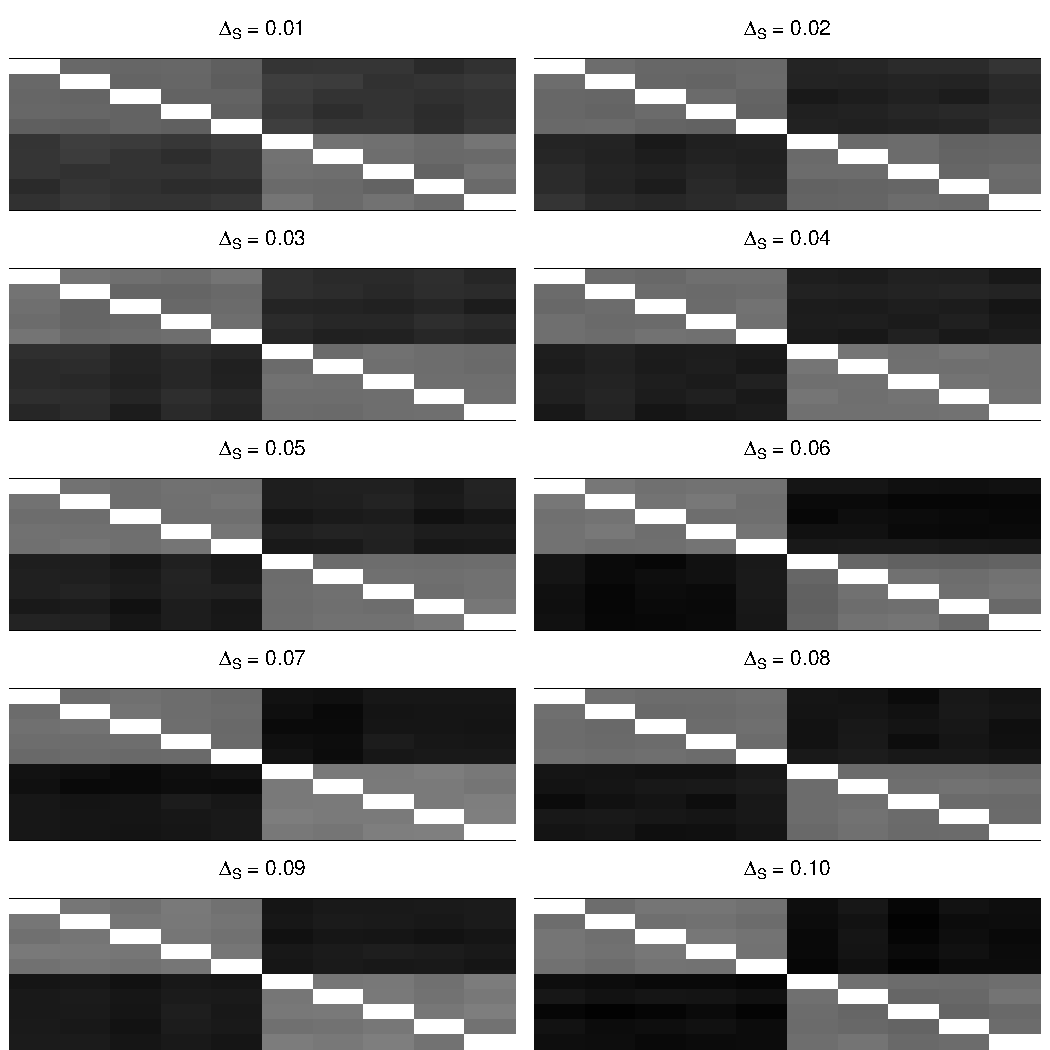
\includegraphics[width=150mm, height=180mm]{figuras/MatBDirecionalIntSel110}
    \caption{Matriz final média de 10 corridas com
        $\mu/\mu_B = 5$, $Ne = 1.000$, $m/p=2$, sofrendo seleção estabilizadora correlacionada com 2
    módulos e seleção direcional com diferentes valores de $\Delta_S$.}
    \label{MatBIntSel110}
\end{figure}

\begin{figure}[htbp]
    \centering
    \subfloat [$\Delta_S = 0.01$]{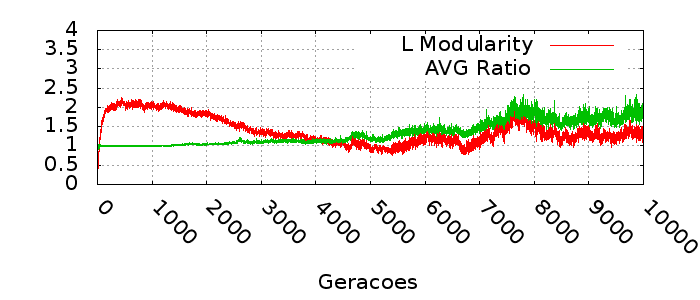
\includegraphics[width=70mm, height=30mm]{figuras/IntSelStats10.png}}\vspace{11pt}
    \subfloat [$\Delta_S = 0.02$]{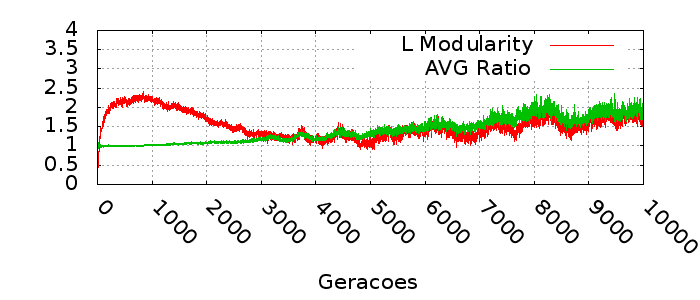
\includegraphics[width=70mm, height=30mm]{figuras/IntSelStats20.png}}\\ 
    \vspace{-18pt}
    \subfloat [$\Delta_S = 0.03$]{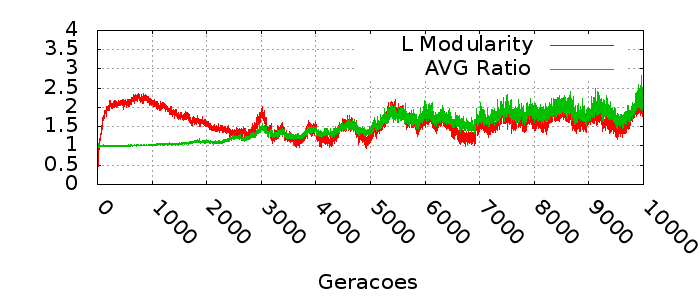
\includegraphics[width=70mm, height=30mm]{figuras/IntSelStats30.png}}\vspace{11pt} 
    \subfloat [$\Delta_S = 0.04$]{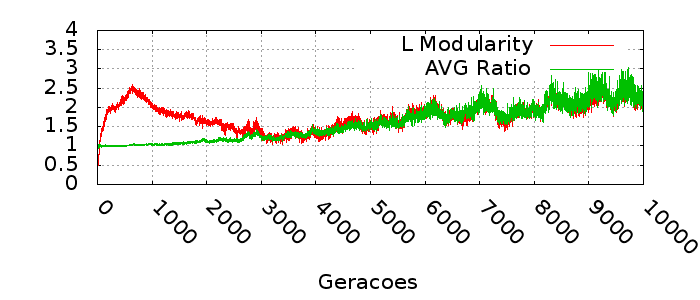
\includegraphics[width=70mm, height=30mm]{figuras/IntSelStats40.png}}\\
    \vspace{-18pt}
    \subfloat [$\Delta_S = 0.05$]{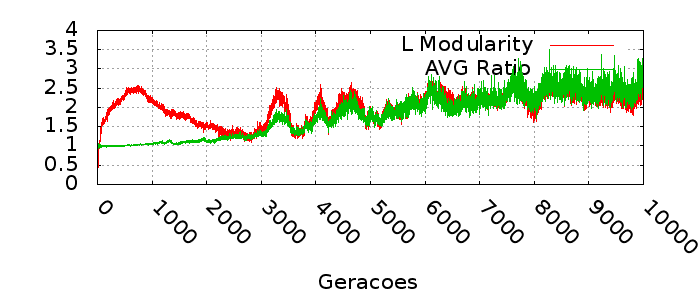
\includegraphics[width=70mm, height=30mm]{figuras/IntSelStats50.png}}\vspace{11pt}
    \subfloat [$\Delta_S = 0.06$]{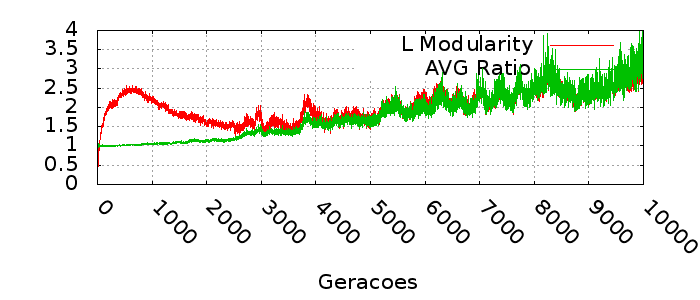
\includegraphics[width=70mm, height=30mm]{figuras/IntSelStats60.png}}\\
    \vspace{-18pt}
    \subfloat [$\Delta_S = 0.07$]{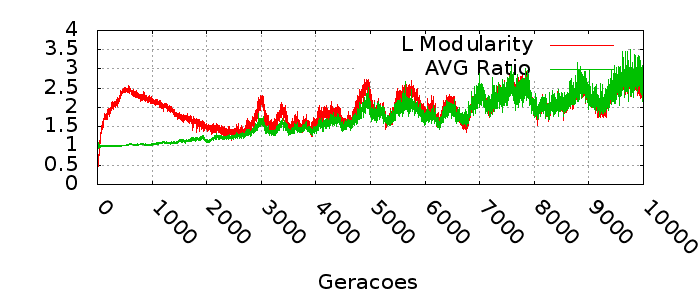
\includegraphics[width=70mm, height=30mm]{figuras/IntSelStats70.png}}\vspace{11pt}
    \subfloat [$\Delta_S = 0.08$]{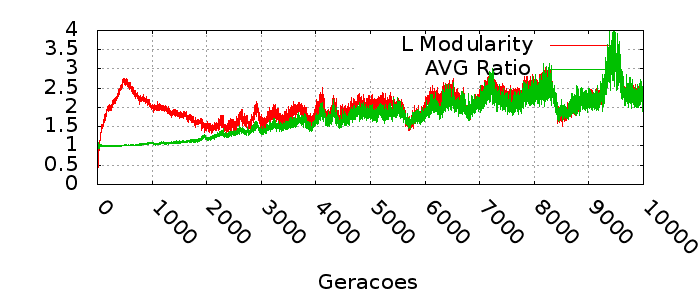
\includegraphics[width=70mm, height=30mm]{figuras/IntSelStats80.png}}\\
    \vspace{-18pt}
    \subfloat [$\Delta_S = 0.09$]{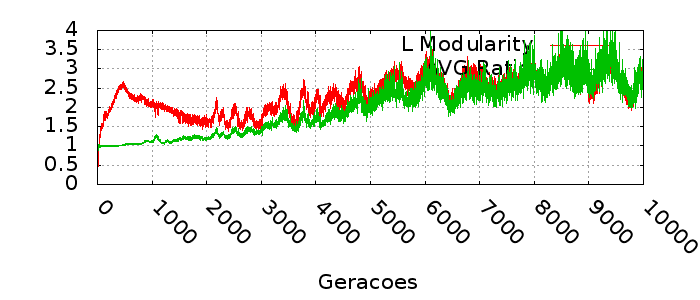
\includegraphics[width=70mm, height=30mm]{figuras/IntSelStats90.png}}\vspace{11pt}
    \subfloat [$\Delta_S = 0.1$]{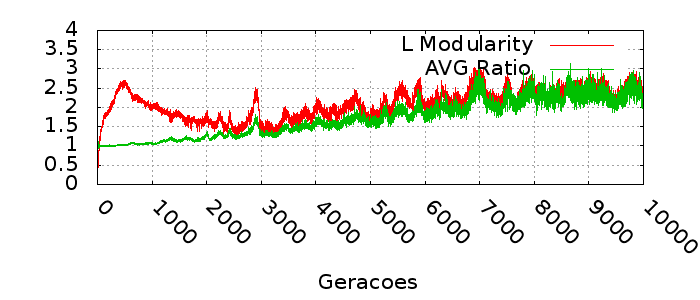
\includegraphics[width=70mm, height=30mm]{figuras/IntSelStats100.png}}\\
    \caption{ AVG-Ratio e modularidade $L$ para corridas com
        $\mu/\mu_B = 5$, $Ne = 2.500$, $m/p=2$, sofrendo seleção
        estabilizadora correlacionada com 2 módulos e seleção direcional com
    diferentes valores de $\Delta_S$.}
    \label{IntSelStats10100}
\end{figure}

\begin{figure}[htbp]
    \centering
    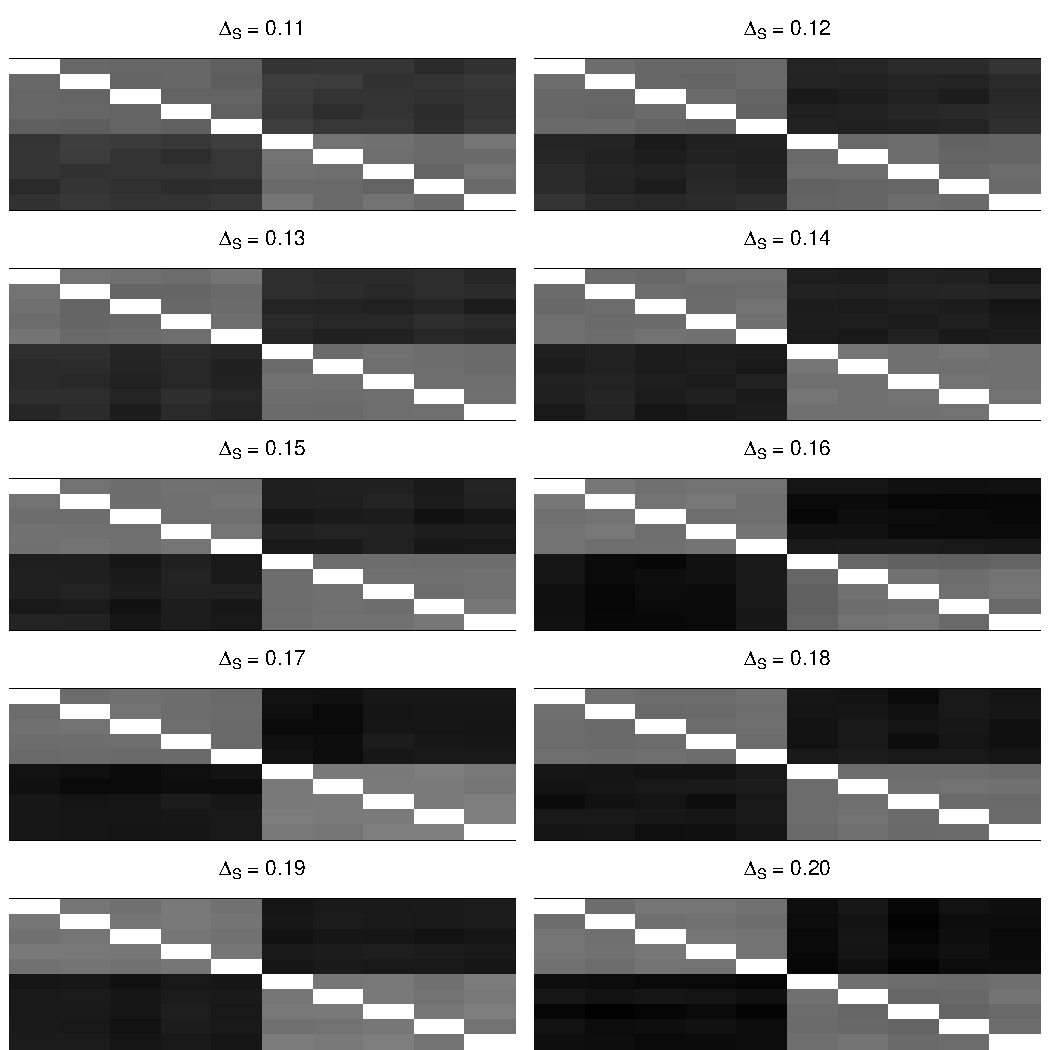
\includegraphics[width=150mm, height=180mm]{figuras/MatBDirecionalIntSel1120}
    \caption{Matriz final média de 10 corridas com
        $\mu/\mu_B = 5$, $Ne = 1.000$, $m/p=2$, sofrendo seleção estabilizadora correlacionada com 2
    módulos e seleção direcional com diferentes valores de $\Delta_S$.}
    \label{MatBIntSel1120}
\end{figure}

\begin{figure}[htbp]
    \centering
    \subfloat [$\Delta_S = 0.11$]{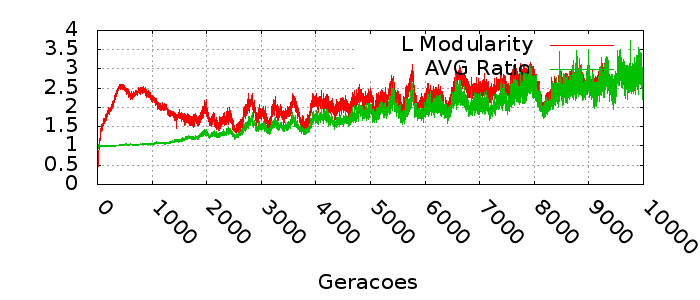
\includegraphics[width=70mm, height=30mm]{figuras/IntSelStats110.png}}\vspace{11pt}
    \subfloat [$\Delta_S = 0.12$]{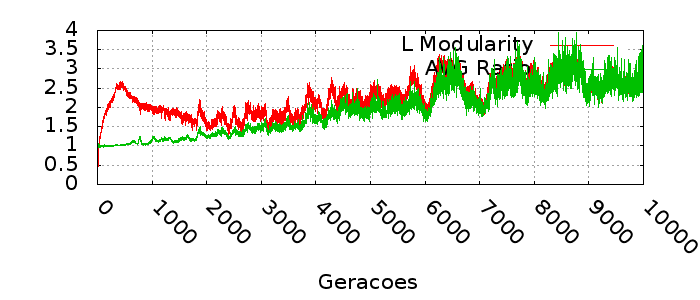
\includegraphics[width=70mm, height=30mm]{figuras/IntSelStats120.png}}\\ 
    \vspace{-18pt}
    \subfloat [$\Delta_S = 0.13$]{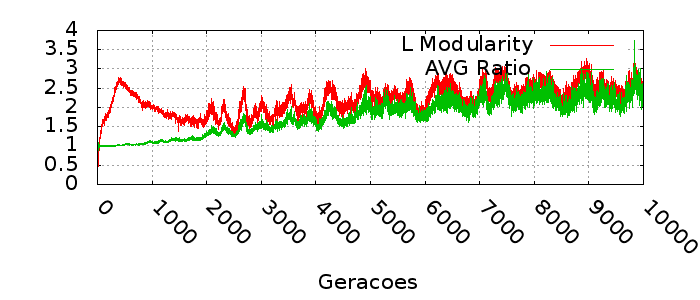
\includegraphics[width=70mm, height=30mm]{figuras/IntSelStats130.png}}\vspace{11pt} 
    \subfloat [$\Delta_S = 0.14$]{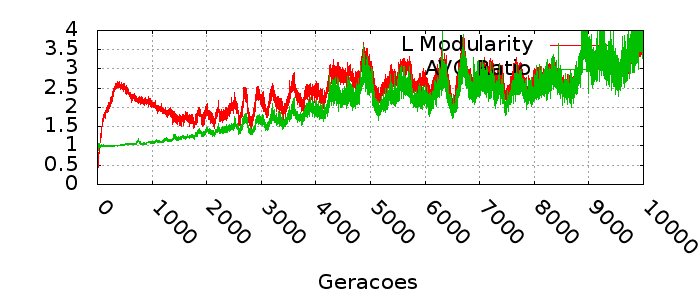
\includegraphics[width=70mm, height=30mm]{figuras/IntSelStats140.png}}\\
    \vspace{-18pt}
    \subfloat [$\Delta_S = 0.15$]{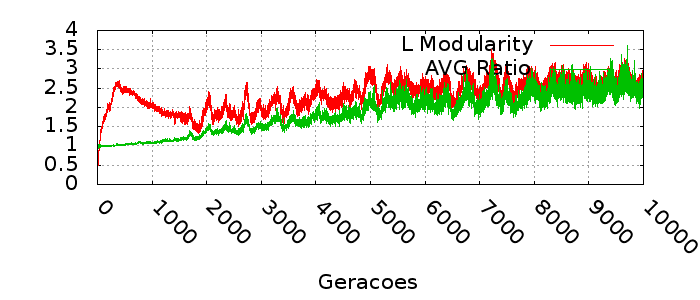
\includegraphics[width=70mm, height=30mm]{figuras/IntSelStats150.png}}\vspace{11pt}
    \subfloat [$\Delta_S = 0.16$]{\includegraphics[width=70mm, height=30mm]{figuras/IntSelStats160.png}}\\
    \vspace{-18pt}
    \subfloat [$\Delta_S = 0.17$]{\includegraphics[width=70mm, height=30mm]{figuras/IntSelStats170.png}}\vspace{11pt}
    \subfloat [$\Delta_S = 0.18$]{\includegraphics[width=70mm, height=30mm]{figuras/IntSelStats180.png}}\\
    \vspace{-18pt}
    \subfloat [$\Delta_S = 0.19$]{\includegraphics[width=70mm, height=30mm]{figuras/IntSelStats190.png}}\vspace{11pt}
    \subfloat [$\Delta_S = 0.2$]{\includegraphics[width=70mm, height=30mm]{figuras/IntSelStats200.png}}\\
    \caption{ AVG-Ratio e modularidade $L$ para corridas com
        $\mu/\mu_B = 5$, $Ne = 2.500$, $m/p=2$, sofrendo seleção
        estabilizadora correlacionada com 2 módulos e seleção direcional com
    diferentes valores de $\Delta_S$.}
    \label{IntSelStats110200}
\end{figure}

\subsection{Seleção direcional seguida de seleção estabilizadora}

Outra questão relevante é o quão estáveis são os padrões de covariação
modulares gerados pela seleção direcional e estabilizadora.
Para responder a essa pergunta nós sujeitamos populações de tamanhos
diferentes a uma mesma pressão seletiva intensa durante 5.000 gerações
(período suficiente para o surgimento de módulos), seguidas de 5.000
gerações de seleção estabilizadora correlacionada.
Apesar da diferença entre as correlações dentro e entre módulos
diminuir, ainda observamos uma distinção estável entre elas (figura
\ref{posselecao} e \ref{posselecaoStats}).
O efeito do tamanho populacional é especialmente marcante nessas
condições, com populações grandes se mostrando mais eficientes na
manutenção prolongada dos padrões estabelecidos pela seleção direcional
(figuras \ref{posselecao} e \ref{posselecaoStats}).

\begin{figure}[htbp]
    \centering
    \subfloat [$Ne = 250$]{\includegraphics[width=70mm, height=50mm]{figuras/posselecao250.png}}\vspace{11pt}
    \subfloat [$Ne = 500$]{\includegraphics[width=70mm, height=50mm]{figuras/posselecao500.png}}\\
    \vspace{-18pt}
    \subfloat [$Ne = 1.000$]{\includegraphics[width=70mm, height=50mm]{figuras/posselecao1000.png}}\vspace{11pt}
    \subfloat [$Ne = 2.500$]{\includegraphics[width=70mm, height=50mm]{figuras/posselecao2500.png}}\\
    \vspace{-18pt}
    \subfloat [$Ne = 5.000$]{\includegraphics[width=70mm, height=50mm]{figuras/posselecao5000.png}}\vspace{11pt}
    \subfloat [$Ne = 10.000$]{\includegraphics[width=70mm, height=50mm]{figuras/posselecao10000.png}}\\
    \caption{Evolução da correlação entre dez caracteres ligados por efeitos
        pleiotrópicos controlados por uma matriz $\mathbf{B}$ variável, sofrendo seleção estabilizadora correlacionada e seleção
        direcional para mudança correlacionada dentro dos módulos
        durante as 5.000 primeiras gerações, seguidos de 5.000 gerações de
    seleção estabilizadora correlacionada ($\Delta_S = 0.2$, $\mu/\mu_B=5$, $m/p=2$).}
    \label{posselecao}
\end{figure}

\begin{figure}[htbp]
    \centering
    \subfloat [$Ne = 250$]{\includegraphics[width=70mm, height=50mm]{figuras/PosSelStatsNe250.png}}\vspace{11pt}
    \subfloat [$Ne = 500$]{\includegraphics[width=70mm, height=50mm]{figuras/PosSelStatsNe500.png}}\\
    \vspace{-18pt}
    \subfloat [$Ne = 1.000$]{\includegraphics[width=70mm, height=50mm]{figuras/PosSelStatsNe1000.png}}\vspace{11pt}
    \subfloat [$Ne = 2.500$]{\includegraphics[width=70mm, height=50mm]{figuras/PosSelStatsNe2500.png}}\\
    \vspace{-18pt}
    \subfloat [$Ne = 5.000$]{\includegraphics[width=70mm, height=50mm]{figuras/PosSelStatsNe5000.png}}\vspace{11pt}
    \subfloat [$Ne = 10.000$]{\includegraphics[width=70mm, height=50mm]{figuras/PosSelStatsNe10000.png}}\\
    \caption{Evolução de modularidade $L$ e AVG-Ratio para as correlações
    apresentadas na figura \ref{posselecao} ($\Delta_S = 0.2$ por $5.000$ gerações, $\mu/\mu_B=5$, $m/p=2$).}
    \label{posselecaoStats}
\end{figure}

\begin{figure}[htbp]
    \centering
    \subfloat [$Ne = 250$]{\includegraphics[width=70mm, height=50mm]{figuras/posselecaoSemEstab250.png}}\vspace{11pt}
    \subfloat [$Ne = 500$]{\includegraphics[width=70mm, height=50mm]{figuras/posselecaoSemEstab500.png}}\\
    \vspace{-18pt}
    \subfloat [$Ne = 1.000$]{\includegraphics[width=70mm, height=50mm]{figuras/posselecaoSemEstab1000.png}}\vspace{11pt}
    \subfloat [$Ne = 2.500$]{\includegraphics[width=70mm, height=50mm]{figuras/posselecaoSemEstab2500.png}}\\
    \vspace{-18pt}
    \subfloat [$Ne = 5.000$]{\includegraphics[width=70mm, height=50mm]{figuras/posselecaoSemEstab5000.png}}\vspace{11pt}
    \subfloat [$Ne = 10.000$]{\includegraphics[width=70mm, height=50mm]{figuras/posselecaoSemEstab10000.png}}\\
    \caption{Evolução da correlação entre dez caracteres ligados por efeitos
        pleiotrópicos controlados por uma matriz $\mathbf{B}$ variável, sofrendo
        seleção estabilizadora correlacionada e seleção direcional para
        mudança correlacionada dentro dos módulos durante as 5.000
        primeiras gerações, seguidos de 5.000 gerações de seleção
        estabilizadora não correlacionada ($\Delta_S = 0.2$, $\mu/\mu_B=5$,
    $m/p=2$).}
    \label{posselecaoSemEstab}
\end{figure}

\begin{figure}[htbp]
    \centering
    \subfloat [$Ne = 250$]{\includegraphics[width=70mm, height=50mm]{figuras/SemEstabPosSelStatsNe250.png}}\vspace{11pt}
    \subfloat [$Ne = 500$]{\includegraphics[width=70mm, height=50mm]{figuras/SemEstabPosSelStatsNe500.png}}\\
    \vspace{-18pt}
    \subfloat [$Ne = 1.000$]{\includegraphics[width=70mm, height=50mm]{figuras/SemEstabPosSelStatsNe1000.png}}\vspace{11pt}
    \subfloat [$Ne = 2.500$]{\includegraphics[width=70mm, height=50mm]{figuras/SemEstabPosSelStatsNe2500.png}}\\
    \vspace{-18pt}
    \subfloat [$Ne = 5.000$]{\includegraphics[width=70mm, height=50mm]{figuras/SemEstabPosSelStatsNe5000.png}}\vspace{11pt}
    \subfloat [$Ne = 10.000$]{\includegraphics[width=70mm, height=50mm]{figuras/SemEstabPosSelStatsNe10000.png}}\\
    \caption{Evolução de modularidade $L$ e AVG-Ratio para as
    correlações apresentadas na figura \ref{posselecaoSemEstab}
    ($\Delta_S = 0.2$ por $5.000$ gerações, $\mu/\mu_B=5$, $m/p=2$).}
    \label{posselecaoSemEstabStats}
\end{figure}

Ainda na questão da estabilidade dos padrões de covariação, o papel da
seleção estabilizadora correlacionada pode ser avaliado sujeitando as
populações à seleção direcional e estabilizadora correlacionada por 5.000
gerações, seguidas de 5.000 gerações de seleção estabilizadora não
correlacionada, apenas mantendo a média de cada caráter individualmente.
Nas figura \ref{posselecaoSemEstab} e \ref{posselecaoSemEstabStats}
podemos ver a importância da seleção estabilizadora correlacionada na
manutenção dos padrões modulares gerados pela seleção direcional.
Comparando cada tamanho populacional mostrado nas figuras
\ref{posselecao}, \ref{posselecaoStats} e \ref{posselecaoSemEstab},
\ref{posselecaoSemEstabStats} podemos ver uma degradação muito mais
acentuada dos padrões modulares na ausência da seleção
estabilizadora correlacionada.
Apesar da diminuição da modularidade, alguma diferenciação entre
correlações dentro e entre módulos se mantém, especialmente nas
populações maiores.
Para $N_e$ acima de $2.500$, e mais marcadamente acima de $5.000$, o
valor de AVG-Ratio se mantém acima de $1.5$ de maneira relativamente
estável, porém o valor de modularidade $L$ decai para $1$.
Para populações suficientemente grandes, apenas seleção estabilizadora
não correlacionada pode ser suficiente para manter modularidade
variacional detectável e com consequências evolutivas, mesmo na ausência
de correlação na superfície de seleção.

A importância da seleção estabilizadora para explicar padrões de estase
no registro fóssil foi amplamente discutida em \cite{Charlesworth1982a}.
No contexto de padrões de covariação, seleção estabilizadora
correlacionada também foi apontada como uma provável explicação para a
estabilidade de padrões de covariação observados na natureza
\citep{Cheverud1984, Marroig2001, Porto2009}.
Nossos resultados dão credibilidade a essa hipótese.
A origem dessa seleção estabilizadora pode ser atribuída a fatores
internos dos organismos, como restrições ontogenéticas responsáveis pela
coesão entre as partes do indivíduo.
Como essas restrições estão sempre presentes, a seleção correlacionada
está sempre presente e os padrões tendem a se manter estáveis.

\subsection{Intensidade de recombinação}

Um parâmetro ainda não mencionado é o número de loci $m$ envolvidos na
determinação do valor fenotípico de cada um dos $p$ caracteres.
No nosso esquema de simulação, aumentar o valor da razão $m/p$ é análogo
a aumentar a força de recombinação, pois o valor de $m$ define o número
de unidades recombinantes segregando na população.
Podemos pensar em $m$ como o número de cromossomos no genoma do
indivíduo (na ausência de recombinação homologa), em vez de pensar nele
como número de alelos individualmente.  Até agora a razão $m/p$ foi
mantida em 2, um valor suficiente para promover respostas complexas de
todos os caracteres mas ainda computacionalmente viável.
Razões maiores de $m/p$ teoricamente aumentam o espaço de variação
possível para população, pois mais genes estão disponíveis para atuar
sobre cada caráter, separadamente ou não.
A figura \ref{MB} mostra como o aumento na razão $m/p$ afeta a evolução
das correlações fenotípicas nas populações sujeitas à seleção direcional
intensa e seleção estabilizadora correlacionada.
Vemos na figura \ref{MB} que o aumento do número de alelos torna o
sistema mais lento em adquirir um caráter modular.
Isso pode ser associado com o aumento na recombinação, que age na
direção oposta a das forças seletivas direcionais e estabilizadora
correlacionada.
Isso nos levou a crer que tempos mais longos de seleção poderiam gerar o
mesmo resultado que o obtido com valores baixos de $m/p$.
Na figura \ref{MBLR} vemos duas corridas longas, de 20.000 gerações, com
$m/p = 9$ e $10$, mostrando o tempo de estabilização mais longo e a
modularidade mais discreta, com menor diferença nas correlações dentro
de e entre módulos.
Isso novamente pode ser explicado pela força de recombinação aumentada.

Praticamente todos os exemplos de surgimento de modularidade mostrados
neste capítulo podem ser interpretados como seleção natural
privilegiando determinados alelos e interações entre alelos que formem
de fenótipos com aptidão maior.
Associações modulares na estrutura genética e aditiva são privilegiadas
por responderem melhor a pressão seletiva imposta.
Porém, essas associações não são herdáveis, apenas os alelos individuais
são passados para a próxima geração.
Isso significa que recombinação pode quebrar as associações criadas pela
seleção, dificultando o estabelecimento da estrutura modular.
Dessa forma, recombinação maior leva a menor eficiência na resposta à
seleção natural.
Essa discussão se encaixa no contexto de alvo e unidade de seleção.
Alvo de seleção é definido como o nível de organização que apresenta o
fenótipo sendo selecionado.
No nosso caso o indivíduo é o único alvo de seleção.
Já a unidade de seleção se refere ao nível de organização genética que
permite prever a resposta à seleção.
Para tal, a unidade de seleção deve ter continuidade entre uma geração e
outra.
Essa definição pode abarcar diferentes níveis, dependendo da estrutura
genética da população.
O alvo de seleção pode ser um único locus ou o genoma todo.
As associações criadas pela seleção natural são exemplos de unidades de
seleção, onde diversos loci interagem para formar um indivíduo com
determinado valor de aptidão.
As associações modulares observadas nos nossos resultados são um
exemplo de unidade de seleção maiores que um locus.
É nesse ponto que a recombinação se torna relevante para definir a
unidade de seleção, pois recombinação age no sentido de quebrar
associação entre loci ao longo das gerações, reduzindo a unidade de
seleção e embaralhando associações modulares.

\centerline { $ * \quad * \quad * $ }

Com isso exploramos algumas das combinações de parâmetros possíveis
nesses modelos, além das suas interpretações e consequências na evolução
do padrão de correlação nas populações simuladas.
No próximo capitulo vamos utilizar combinações plausíveis de parâmetros
no nosso modelo para testar a viabilidade de trajetórias evolutivas que
levem a modularidade variacional.

\begin{figure}[htbp]
    \centering
    \subfloat [$m/p = 2$]{\includegraphics[width=70mm, height=40mm]{figuras/MB20.png}}\vspace{11pt}
    \subfloat [$m/p = 3$]{\includegraphics[width=70mm, height=40mm]{figuras/MB30.png}}\\
    \vspace{-18pt}
    \subfloat [$m/p = 4$]{\includegraphics[width=70mm, height=40mm]{figuras/MB40.png}}\vspace{11pt}
    \subfloat [$m/p = 5$]{\includegraphics[width=70mm, height=40mm]{figuras/MB50.png}}\\
    \vspace{-18pt}
    \subfloat [$m/p = 6$]{\includegraphics[width=70mm, height=40mm]{figuras/MB60.png}}\vspace{11pt}
    \subfloat [$m/p = 7$]{\includegraphics[width=70mm, height=40mm]{figuras/MB70.png}}\\
    \vspace{-18pt}
    \subfloat [$m/p = 8$]{\includegraphics[width=70mm, height=40mm]{figuras/MB80.png}}\vspace{11pt}
    \subfloat [$m/p = 9$]{\includegraphics[width=70mm, height=40mm]{figuras/MB90.png}}\\
    \caption{Evolução da correlação entre dez caracteres ligados por efeitos
        pleiotrópicos controlados por uma função ontogenética linear binária
        variável sofrendo seleção estabilizadora correlacionada e seleção
        direcional intensa para mudança correlacionada dentro dos módulos,
        para diferentes valores do número de loci. ($Ne=5.000$, $\mu/\mu_B=5$, $\Delta_S=0.2$)}
    \label{MB}
\end{figure}

\begin{figure}[htbp]
    \centering
    \subfloat [$m/p = 9$]{\includegraphics[width=150mm, height=80mm]{figuras/MBLR90.png}}\vspace{11pt}
    \vspace{-18pt}
    \subfloat [$m/p = 10$]{\includegraphics[width=150mm, height=80mm]{figuras/MBLR100.png}}\vspace{11pt}
    \caption{Evolução da correlação entre dez caracteres ligados por efeitos
        pleiotrópicos controlados por uma função ontogenética linear binária
        variável sofrendo seleção estabilizadora correlacionada e seleção
        direcional intensa para mudança correlacionada dentro dos módulos,
        para diferentes valores do número de loci. ($Ne=5.000$, $\mu/\mu_B=5$, $\Delta_S=0.2$)}
    \label{MBLR}
\end{figure}

